\documentclass[11pt]{article}
\usepackage[margin=0.9in]{geometry}
\usepackage[utf8]{inputenc}
\usepackage[T1]{fontenc}
\usepackage{graphicx}
\usepackage{booktabs}
\usepackage{array}
\usepackage{xcolor}
\usepackage{listings}
\usepackage{hyperref}
\usepackage{parskip}
\definecolor{codebg}{RGB}{245,245,245}
\lstset{basicstyle=\ttfamily\footnotesize, backgroundcolor=\color{codebg},
  breaklines=true, frame=single, columns=fullflexible, keepspaces=true,
  showstringspaces=false}
% HW6 formatting rule: main headings 14 pt bold, subheadings 12 pt bold, body 11 pt
\makeatletter
\renewcommand\section{\@startsection{section}{1}{\z@}{-3.0ex \@plus -1ex \@minus -.2ex}{1.2ex \@plus.2ex}{\normalfont\fontsize{14}{17}\selectfont\bfseries}}
\renewcommand\subsection{\@startsection{subsection}{2}{\z@}{-2.2ex \@plus -1ex \@minus -.2ex}{0.8ex \@plus.2ex}{\normalfont\fontsize{12}{14.5}\selectfont\bfseries}}
\makeatother
\emergencystretch=3em

\title{DATA-260 Homework 6 -- Report}
\author{Uday Patel}
\date{}

\begin{document}
\maketitle

\section*{Section 0 -- Personal Configuration and Domain}
\begin{tabular}{|l|l|}\hline
\textbf{Value} & \textbf{Result} \\\hline
SID4 & 9871 \\\hline
PORT\_BASE & 8871 \\\hline
PREFIX & s9871 \\\hline
SEED & 9871 \\\hline
VERIFY\_SEED & 269871 \\\hline
DOMAIN\_ID & 7 -- Community sports league fixtures \\\hline
\end{tabular}
\vspace{1em}

\textbf{Hardware:} Lenovo Legion Slim 5 16" (Ryzen 5 7640HS, 16GB RAM, RTX 4060 8GB, 512GB SSD). \\
\textbf{Local model used:} qwen3:8b via Ollama (thinking disabled, temperature 0.3, sampling seed 9871) for chat replies, summaries, episode extraction and memory consolidation; sentence-transformers/all-MiniLM-L6-v2 for episode embeddings. \\
\textbf{Repository:} \url{https://github.com/UdayPate/data260-9871} \\
\textbf{Tagged commit:} PLACEHOLDER\_HASH (to be filled in after the final commit and hw6 tag) \\
{\footnotesize\url{https://github.com/UdayPate/data260-9871/tree/PLACEHOLDER_HASH}} \\
\textbf{Collaborator access:} confirmed working for Sbnikitha and supriyaselvanganesan.

\section*{Part 1 -- MongoDB Document API}
Added a MongoDB-backed document view of the fixtures domain in the shared \verb|code/doc_api/| package (separate files: \verb|config.py|, \verb|db.py| PyMongo connection, \verb|schemas.py| Pydantic models, \verb|routes.py| handlers, \verb|main.py| server). Database \verb|s9871_doc|, collection \verb|fixtures|.
\subsection*{I. Database}
Required short text field (max 100), optional description, two constrained fields (\verb|status| with default \verb|scheduled|, \verb|category| with four sports), a required date/time, and automatic created/updated timestamps. Validation is enforced twice: by Pydantic in the API and by a MongoDB \verb|$jsonSchema| validator in the database itself.
\textbf{Connection and settings.} \verb|config.py| holds the fixed values, \verb|db.py| creates one shared PyMongo client and installs the collection validator plus indexes at startup (\verb|init_db| is idempotent: it creates the collection with the validator, or updates it with \verb|collMod| if it already exists). \verb|tz_aware=True| makes dates round-trip as UTC.
\begingroup\lstset{basicstyle=\ttfamily\scriptsize}
\begin{lstlisting}
SID4 = "9871"
PREFIX = "s9871"
PORT_BASE = 8871
SEED = 9871
VERIFY_SEED = 269871

MONGO_URI = os.environ.get("MONGO_URI", "mongodb://localhost:27017")
MONGO_DB = f"{PREFIX}_doc"
FIXTURES_COLLECTION = "fixtures"
CORS_ORIGINS = ["http://localhost:5173", f"http://localhost:{PORT_BASE}"]
\end{lstlisting}
\endgroup
\begingroup\lstset{basicstyle=\ttfamily\scriptsize}
\begin{lstlisting}
CATEGORIES = ["Soccer", "Basketball", "Volleyball", "Cricket"]

STATUSES = ["scheduled", "in_progress", "completed", "cancelled"]

def get_client() -> MongoClient:
    global _client
    if _client is None:
        _client = MongoClient(config.MONGO_URI, serverSelectionTimeoutMS=3000, tz_aware=True)
    return _client

def get_db():
    return get_client()[config.MONGO_DB]

def fixtures():
    return get_db()[config.FIXTURES_COLLECTION]

def init_db() -> None:
    """Create the fixtures collection with its validator (idempotent)."""
    db = get_db()
    name = config.FIXTURES_COLLECTION
    if name not in db.list_collection_names():
        db.create_collection(name, validator=FIXTURE_VALIDATOR,
                             validationLevel="strict", validationAction="error")
    else:
        db.command("collMod", name, validator=FIXTURE_VALIDATOR,
                   validationLevel="strict", validationAction="error")
    _init_memory_collections(db)
    db[name].create_index([("match_date", ASCENDING)])
    db[name].create_index([("category", ASCENDING), ("status", ASCENDING)])
\end{lstlisting}
\endgroup
\textbf{Pydantic models} (the first line of defence: required fields, length limits, enums, date parsing, and \verb|extra=forbid| to reject unknown fields):
\begingroup\lstset{basicstyle=\ttfamily\scriptsize}
\begin{lstlisting}
class Category(str, Enum):
    soccer = "Soccer"
    basketball = "Basketball"
    volleyball = "Volleyball"
    cricket = "Cricket"

class Status(str, Enum):
    scheduled = "scheduled"
    in_progress = "in_progress"
    completed = "completed"
    cancelled = "cancelled"

class FixtureCreate(BaseModel):
    model_config = ConfigDict(extra="forbid")

    fixture_name: str = Field(..., min_length=1, max_length=100)
    description: Optional[str] = Field(None, max_length=2000)
    status: Status = Status.scheduled
    category: Category
    match_date: datetime

    @field_validator("fixture_name")
    @classmethod
    def _not_blank(cls, v: str) -> str:
        v = v.strip()
        if not v:
            raise ValueError("fixture_name must not be blank")
        return v

class FixtureOut(BaseModel):
    id: str
    fixture_name: str
    description: Optional[str] = None
    status: Status
    category: Category
    match_date: datetime
    created_at: datetime
    updated_at: datetime
\end{lstlisting}
\endgroup
\textbf{Database-level validator} (the backstop: MongoDB itself rejects a bad document even if something bypasses the API):
\begingroup\lstset{basicstyle=\ttfamily\scriptsize}
\begin{lstlisting}
FIXTURE_VALIDATOR = {
    "$jsonSchema": {
        "bsonType": "object",
        "required": ["fixture_name", "status", "category", "match_date",
                     "created_at", "updated_at"],
        "properties": {
            "fixture_name": {"bsonType": "string", "minLength": 1, "maxLength": 100},
            "description": {"bsonType": "string", "maxLength": 2000},
            "status": {"enum": STATUSES},
            "category": {"enum": CATEGORIES},
            "match_date": {"bsonType": "date"},
            "created_at": {"bsonType": "date"},
            "updated_at": {"bsonType": "date"},
        },
    }
}
\end{lstlisting}
\endgroup
\begin{center}
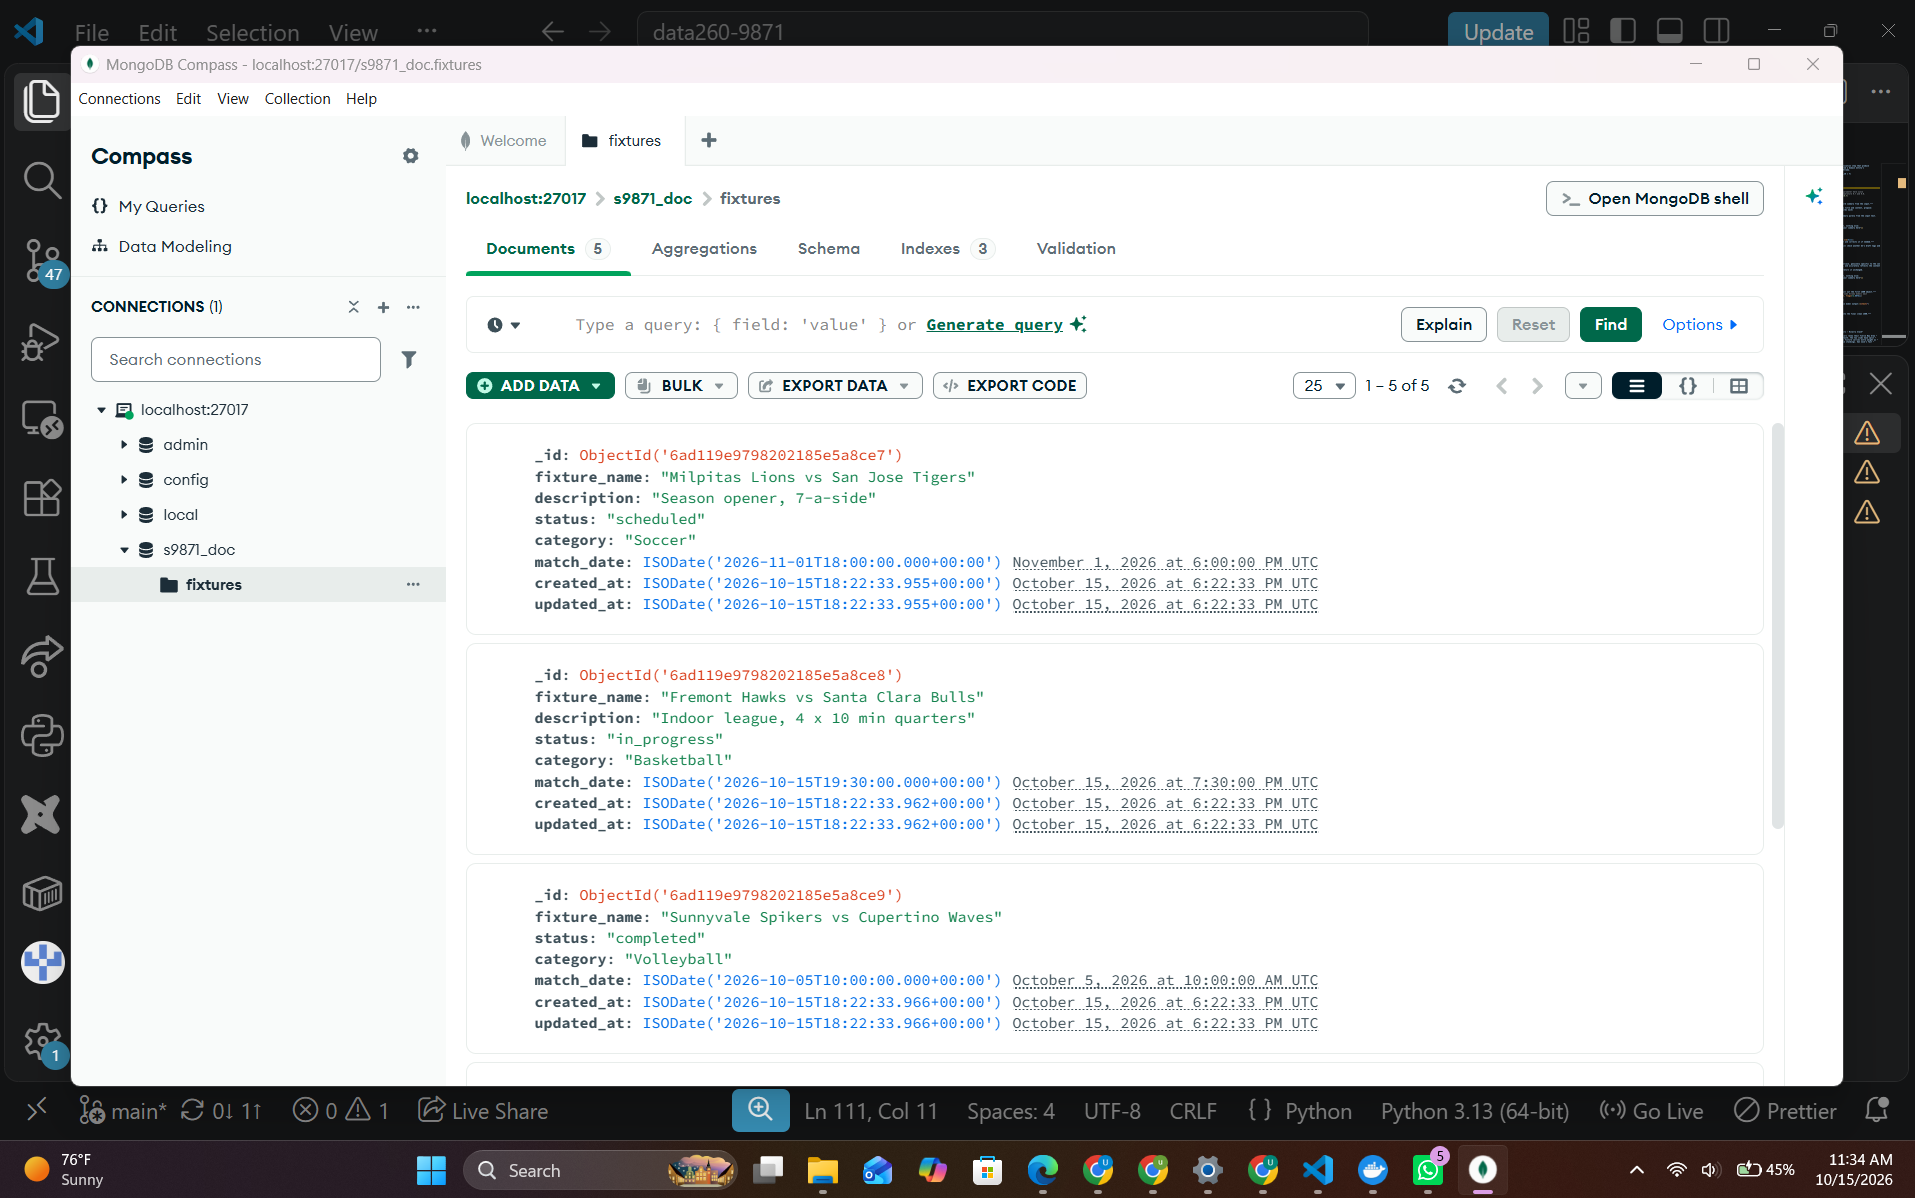
\includegraphics[width=0.80\linewidth,height=0.34\textheight,keepaspectratio]{screenshots/part1_compass_fixtures.png}\\[2pt]
\small \textit{Figure 1: MongoDB Compass: \texttt{s9871\_doc.fixtures} with the 5 sample documents.}
\end{center}
\begin{center}
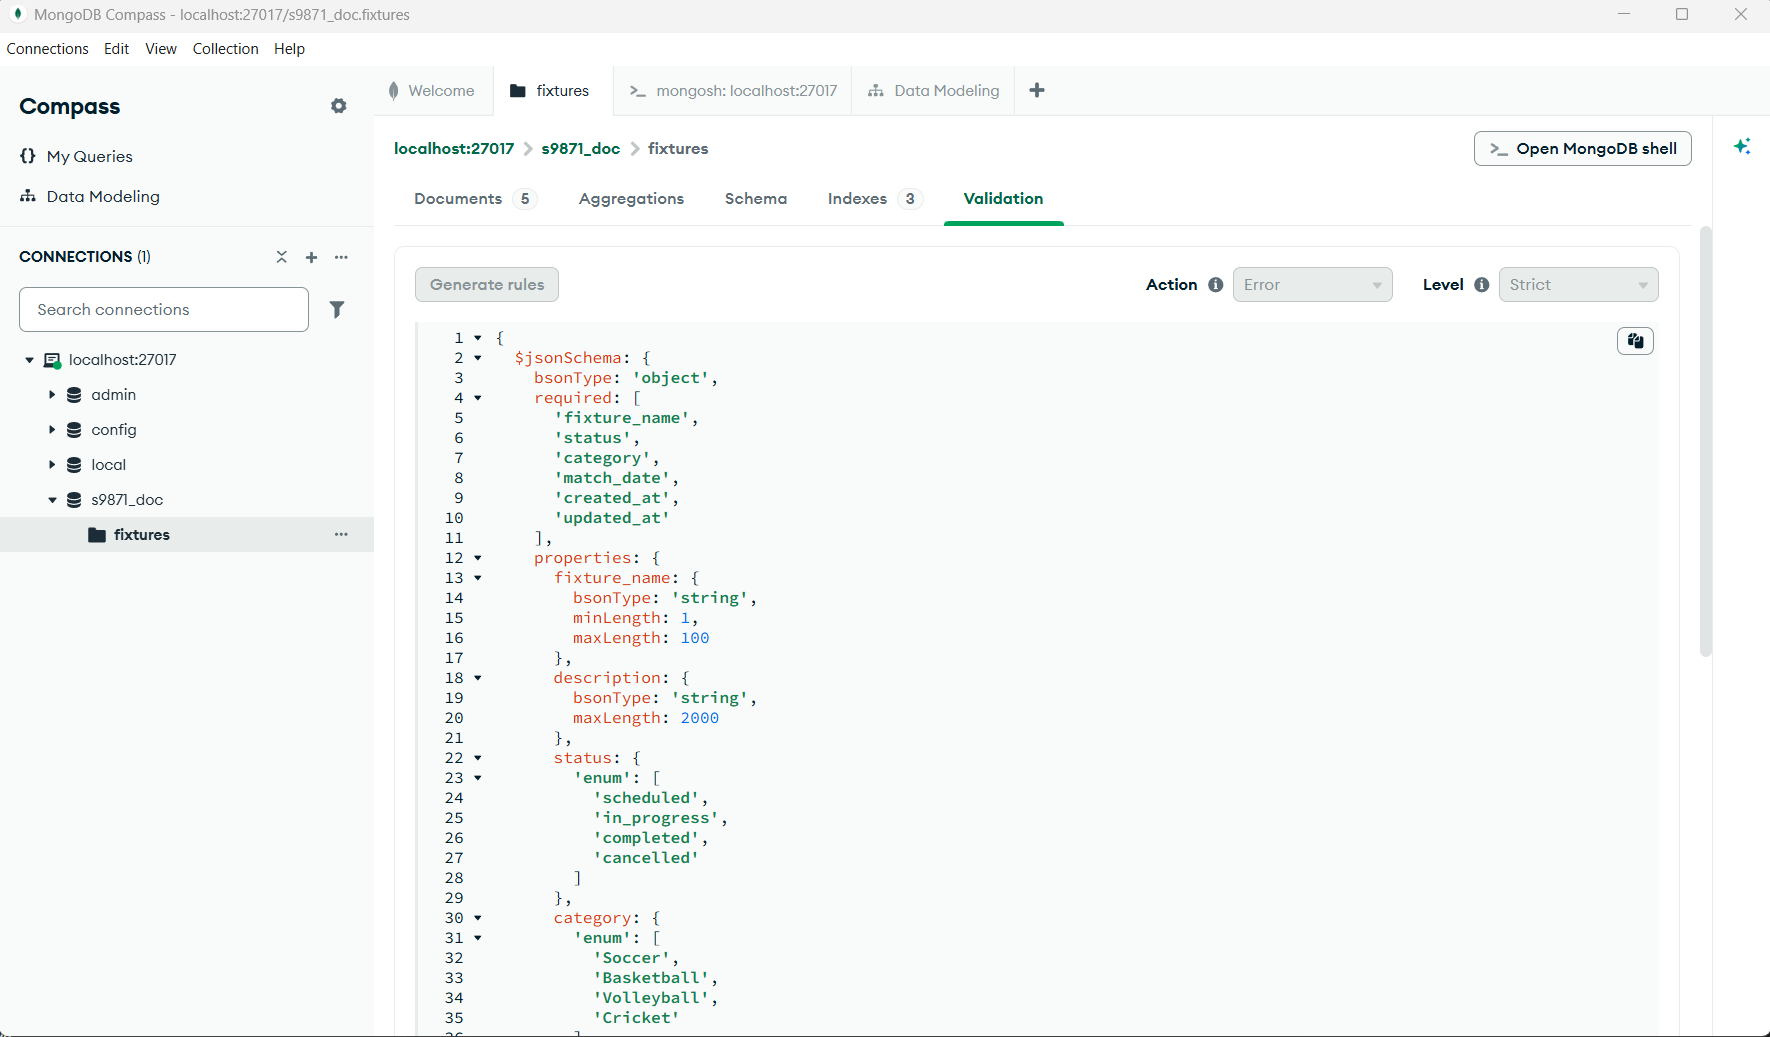
\includegraphics[width=0.80\linewidth,height=0.32\textheight,keepaspectratio]{screenshots/part1_compass_validation.png}\\[2pt]
\small \textit{Figure 2: Compass Validation tab showing the \texttt{\$jsonSchema} rules (required fields, maxLength 100, enums; Action=Error, Level=Strict).}
\end{center}
\subsection*{II. API implementation}
Full CRUD with proper status codes (201, 200, 204, 404 unknown id, 400 malformed id, 422 invalid data, 503 database error, 500 unexpected). CORS middleware is added in \verb|main.py|; JSON request bodies are parsed by FastAPI/Pydantic.
The handlers share three small helpers: \verb|_oid| turns a bad id into a 400, \verb|_out| maps a Mongo document to the response model, and \verb|_payload| builds the stored document. The five CRUD handlers:
\begingroup\lstset{basicstyle=\ttfamily\scriptsize}
\begin{lstlisting}
def _oid(raw: str) -> ObjectId:
    try:
        return ObjectId(raw)
    except (InvalidId, TypeError):
        raise HTTPException(status_code=400, detail=f"'{raw}' is not a valid fixture id")

def _out(doc: dict) -> FixtureOut:
    doc = dict(doc)
    doc["id"] = str(doc.pop("_id"))
    return FixtureOut(**doc)

def _payload(model) -> dict:
    data = model.model_dump(mode="python")
    data["status"] = model.status.value
    data["category"] = model.category.value
    if data.get("description") is None:
        data.pop("description", None)
    return data
\end{lstlisting}
\endgroup
\begingroup\lstset{basicstyle=\ttfamily\scriptsize}
\begin{lstlisting}
def create_fixture(body: FixtureCreate):
    now = datetime.now(timezone.utc)
    doc = {**_payload(body), "created_at": now, "updated_at": now}
    try:
        res = db.fixtures().insert_one(doc)
    except WriteError as exc:
        raise HTTPException(status_code=422, detail=f"database validation failed: {exc}")
    doc["_id"] = res.inserted_id
    return _out(doc)

def list_fixtures():
    return [_out(d) for d in db.fixtures().find().sort("match_date", 1)]

def get_fixture(fixture_id: str):
    doc = db.fixtures().find_one({"_id": _oid(fixture_id)})
    if doc is None:
        raise HTTPException(status_code=404, detail="fixture not found")
    return _out(doc)

def update_fixture(fixture_id: str, body: FixtureUpdate):
    data = _payload(body)
    update = {"$set": {**data, "updated_at": datetime.now(timezone.utc)}}
    if "description" not in data:
        update["$unset"] = {"description": ""}
    try:
        doc = db.fixtures().find_one_and_update(
            {"_id": _oid(fixture_id)}, update, return_document=ReturnDocument.AFTER)
    except WriteError as exc:
        raise HTTPException(status_code=422, detail=f"database validation failed: {exc}")
    if doc is None:
        raise HTTPException(status_code=404, detail="fixture not found")
    return _out(doc)

def delete_fixture(fixture_id: str):
    res = db.fixtures().delete_one({"_id": _oid(fixture_id)})
    if res.deleted_count == 0:
        raise HTTPException(status_code=404, detail="fixture not found")
    return Response(status_code=204)
\end{lstlisting}
\endgroup
Server configuration (\verb|main.py|): startup creates the collections, CORS middleware, and the handlers that turn database failures into 503 and anything unexpected into a 500 instead of a stack trace.
\begingroup\lstset{basicstyle=\ttfamily\scriptsize}
\begin{lstlisting}
async def lifespan(_app: FastAPI):
    db.init_db()
    yield
\end{lstlisting}
\endgroup
\begingroup\lstset{basicstyle=\ttfamily\footnotesize}
\begin{lstlisting}
app.add_middleware(
    CORSMiddleware,
    allow_origins=config.CORS_ORIGINS,
    allow_credentials=True,
    allow_methods=["*"],
    allow_headers=["*"],
)
\end{lstlisting}
\endgroup
\begingroup\lstset{basicstyle=\ttfamily\scriptsize}
\begin{lstlisting}
async def mongo_handler(request: Request, exc: PyMongoError):
    log.exception("database error")
    return JSONResponse(status_code=503, content={"detail": "database unavailable or failed"})

async def unhandled_handler(request: Request, exc: Exception):
    log.exception("unhandled error")
    return JSONResponse(status_code=500, content={"detail": "internal server error"})

def health():
    db.get_client().admin.command("ping")
    return {"status": "ok", "db": config.MONGO_DB}
\end{lstlisting}
\endgroup
\begin{center}
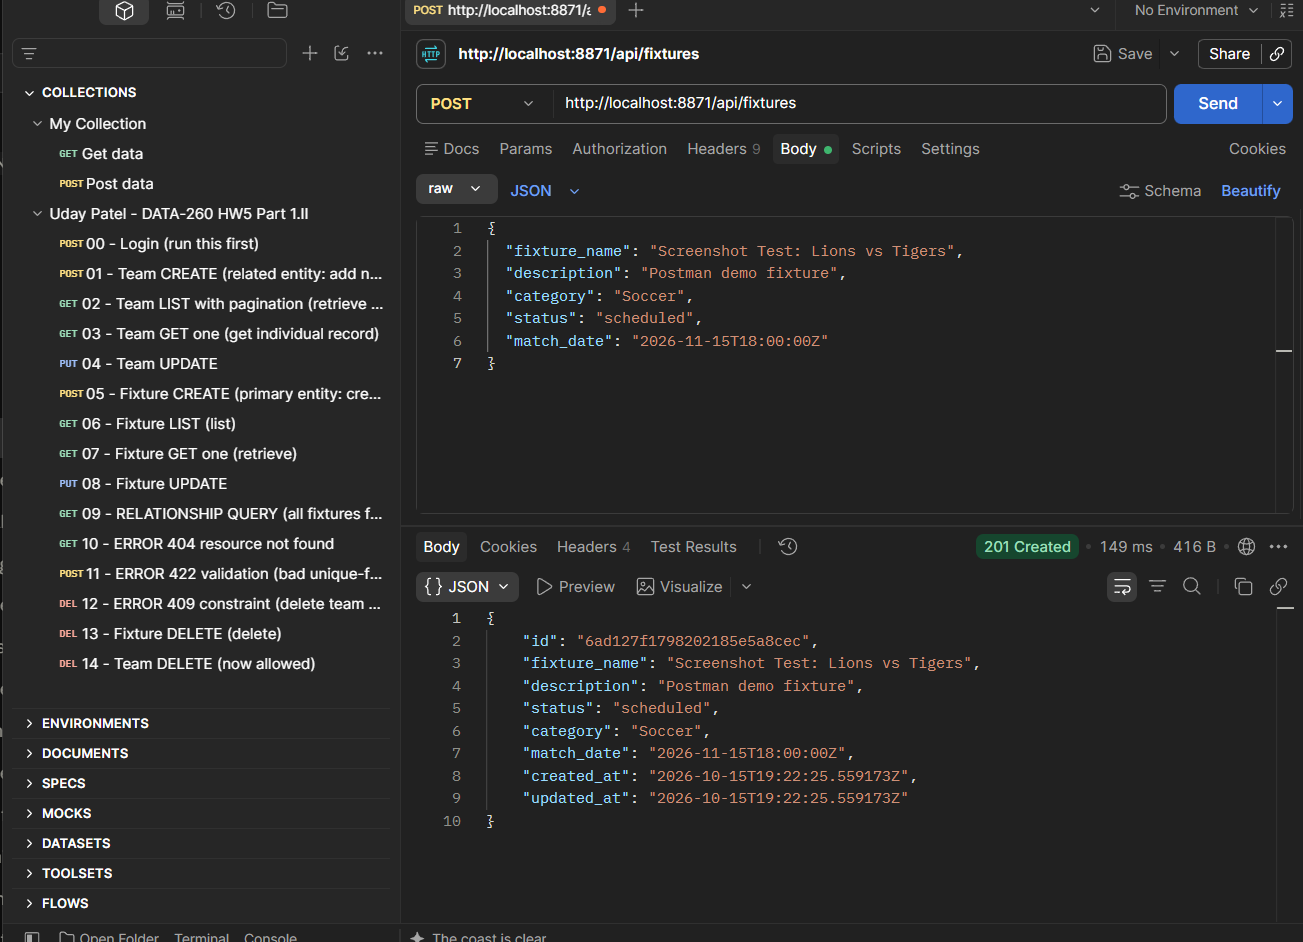
\includegraphics[width=0.80\linewidth,height=0.34\textheight,keepaspectratio]{screenshots/part1_post_create.png}\\[2pt]
\small \textit{Figure 3: POST /api/fixtures: 201 Created, default status, matching created/updated timestamps.}
\end{center}
\begin{center}
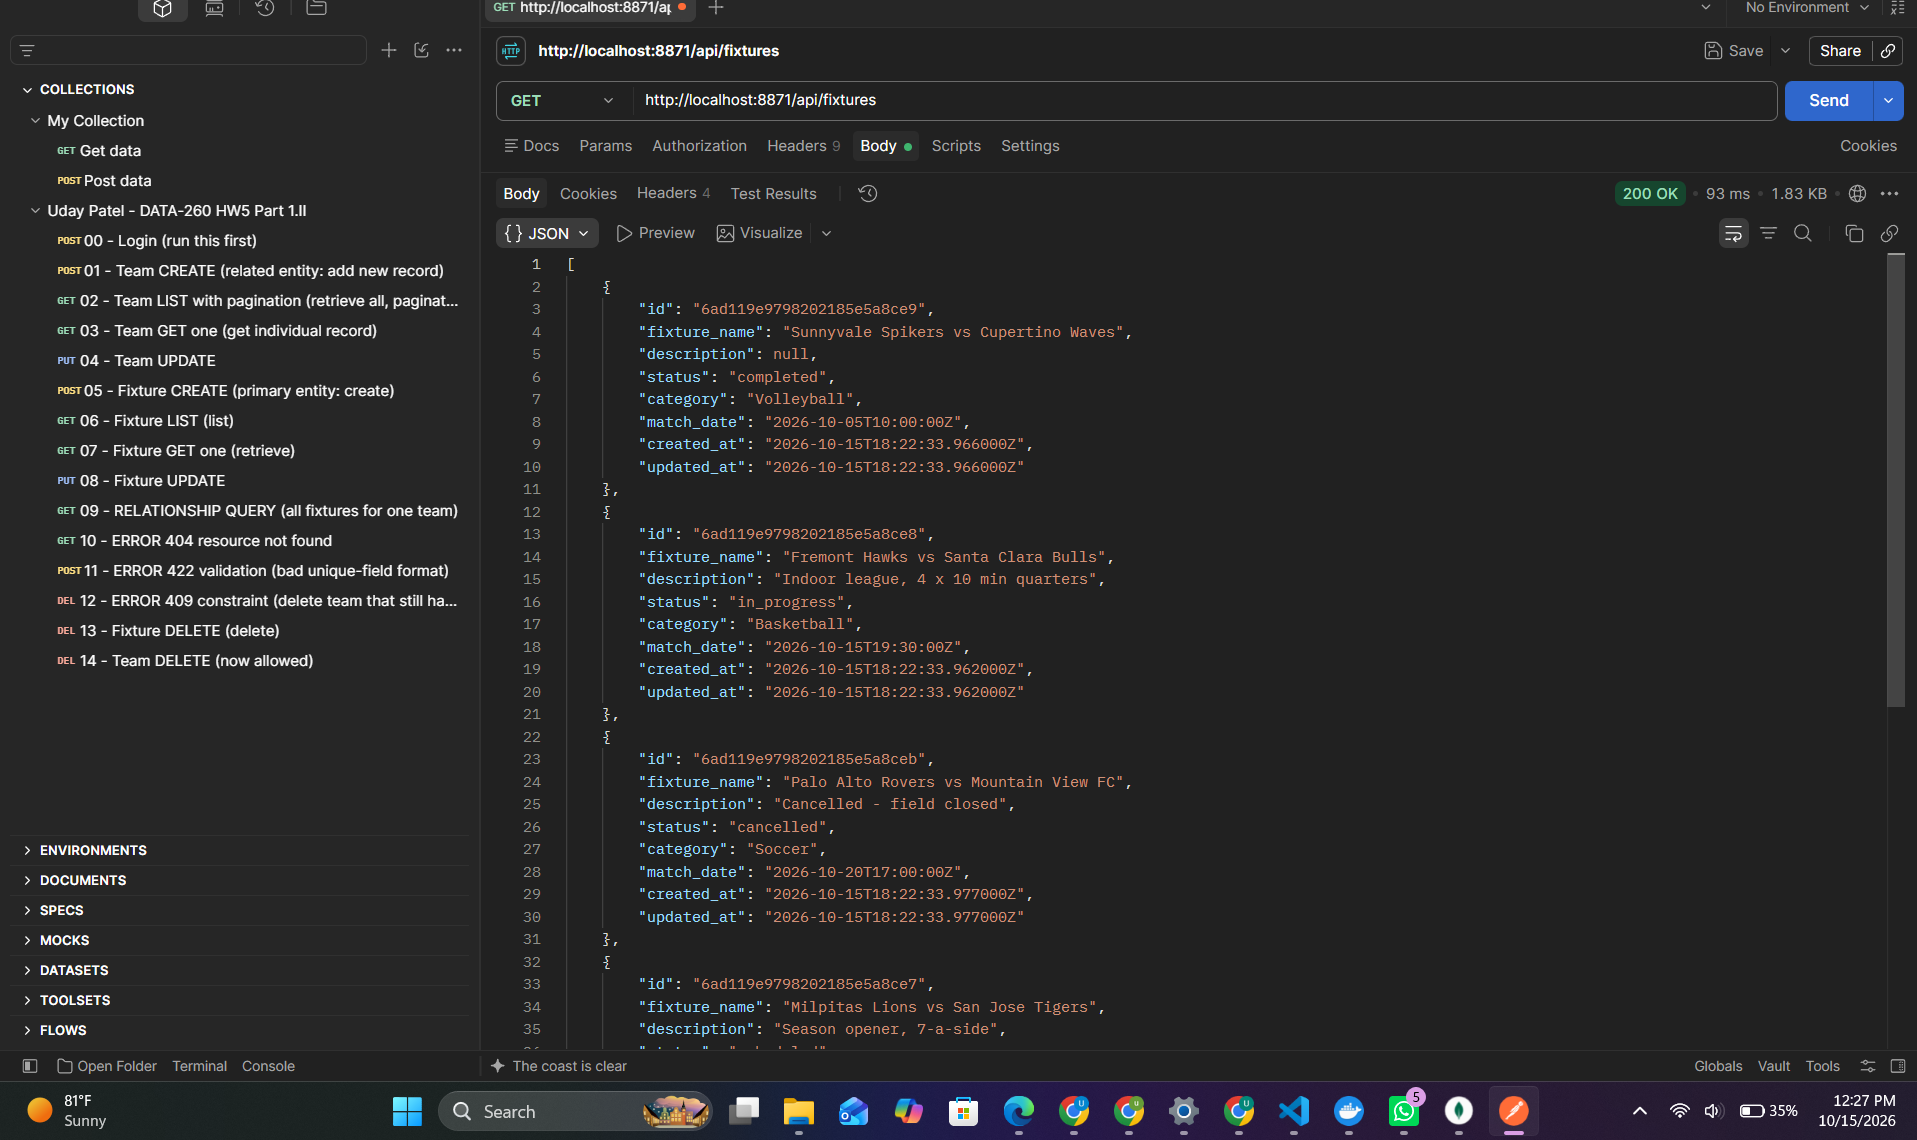
\includegraphics[width=0.80\linewidth,height=0.32\textheight,keepaspectratio]{screenshots/part1_get_all.png}\\[2pt]
\small \textit{Figure 4: GET /api/fixtures: 200 OK, list of fixtures.}
\end{center}
\begin{center}
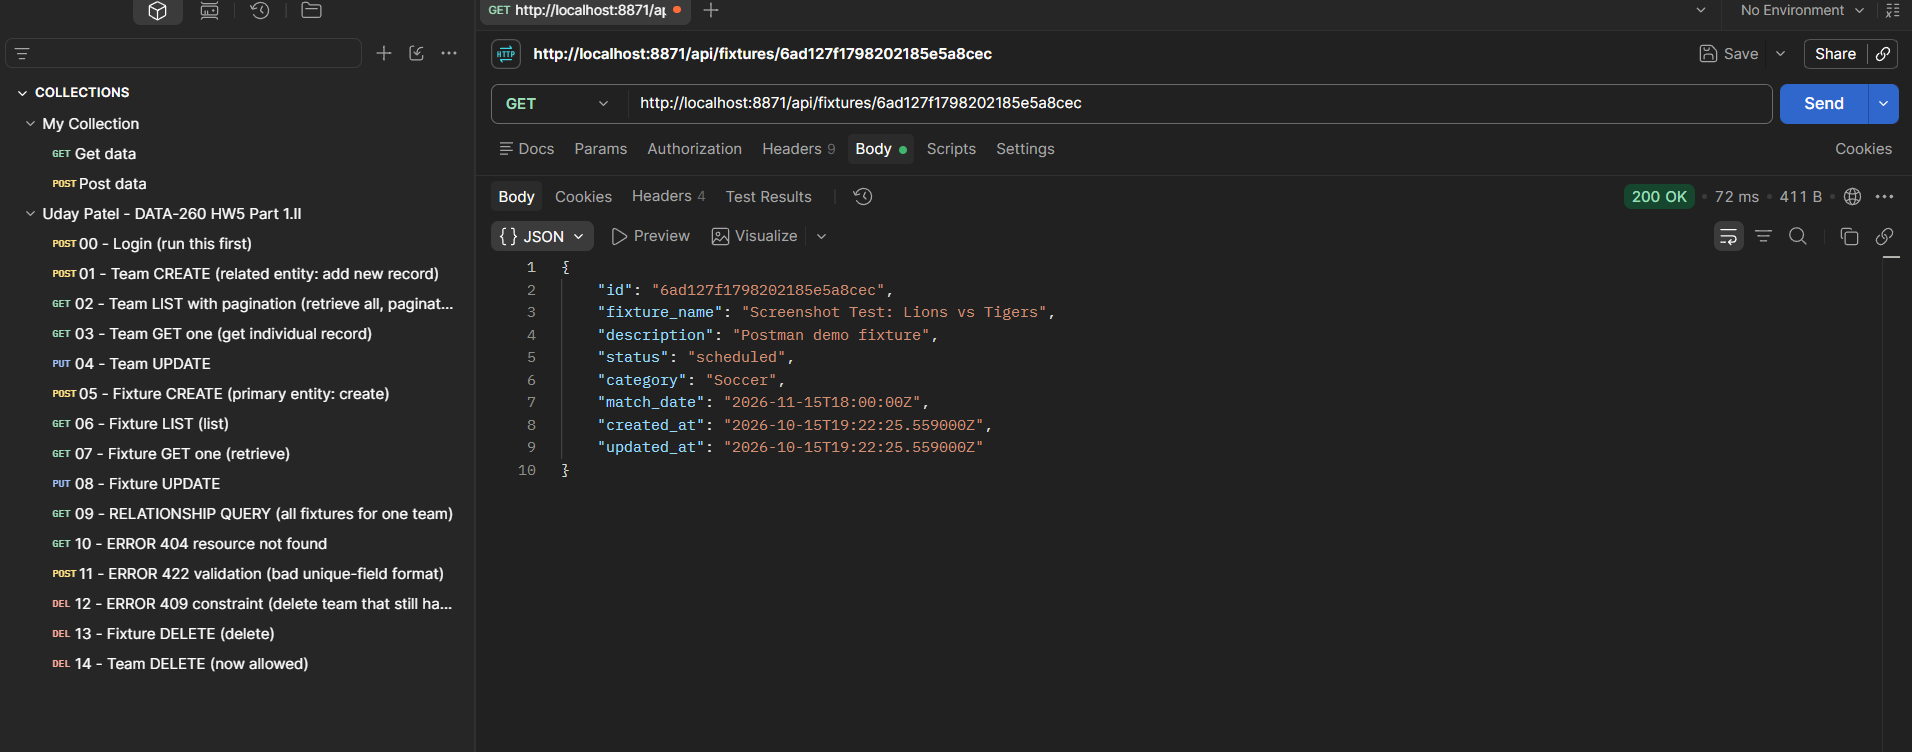
\includegraphics[width=0.80\linewidth,height=0.30\textheight,keepaspectratio]{screenshots/part1_get_one.png}\\[2pt]
\small \textit{Figure 5: GET /api/fixtures/\{id\}: 200 OK.}
\end{center}
\begin{center}
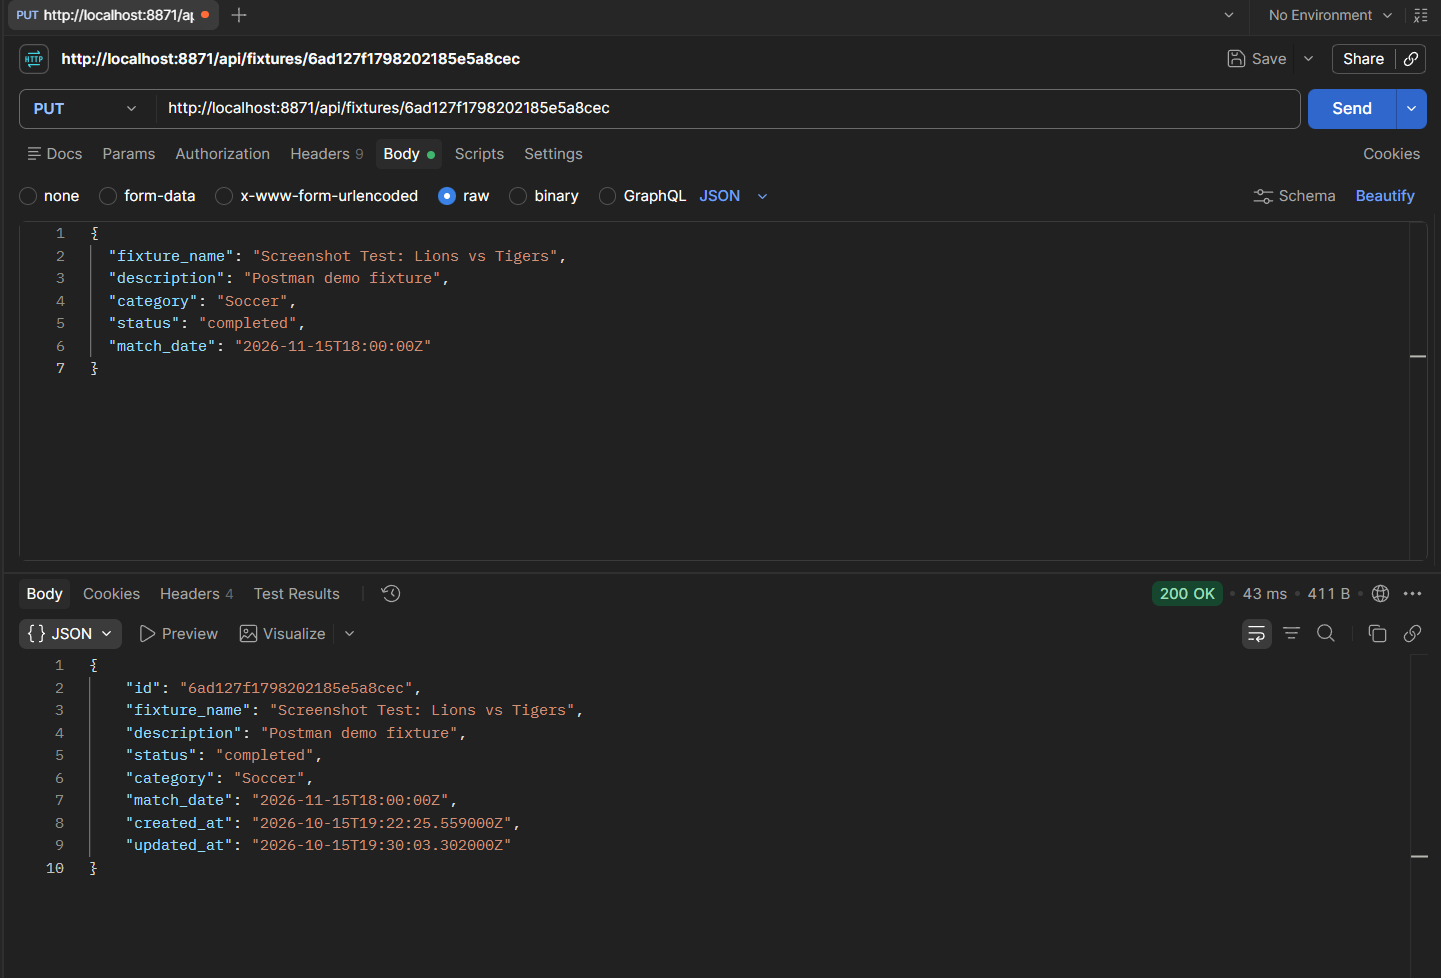
\includegraphics[width=0.80\linewidth,height=0.34\textheight,keepaspectratio]{screenshots/part1_put_update.png}\\[2pt]
\small \textit{Figure 6: PUT /api/fixtures/\{id\}: 200 OK, new status, \texttt{updated\_at} later than \texttt{created\_at}.}
\end{center}
\begin{center}
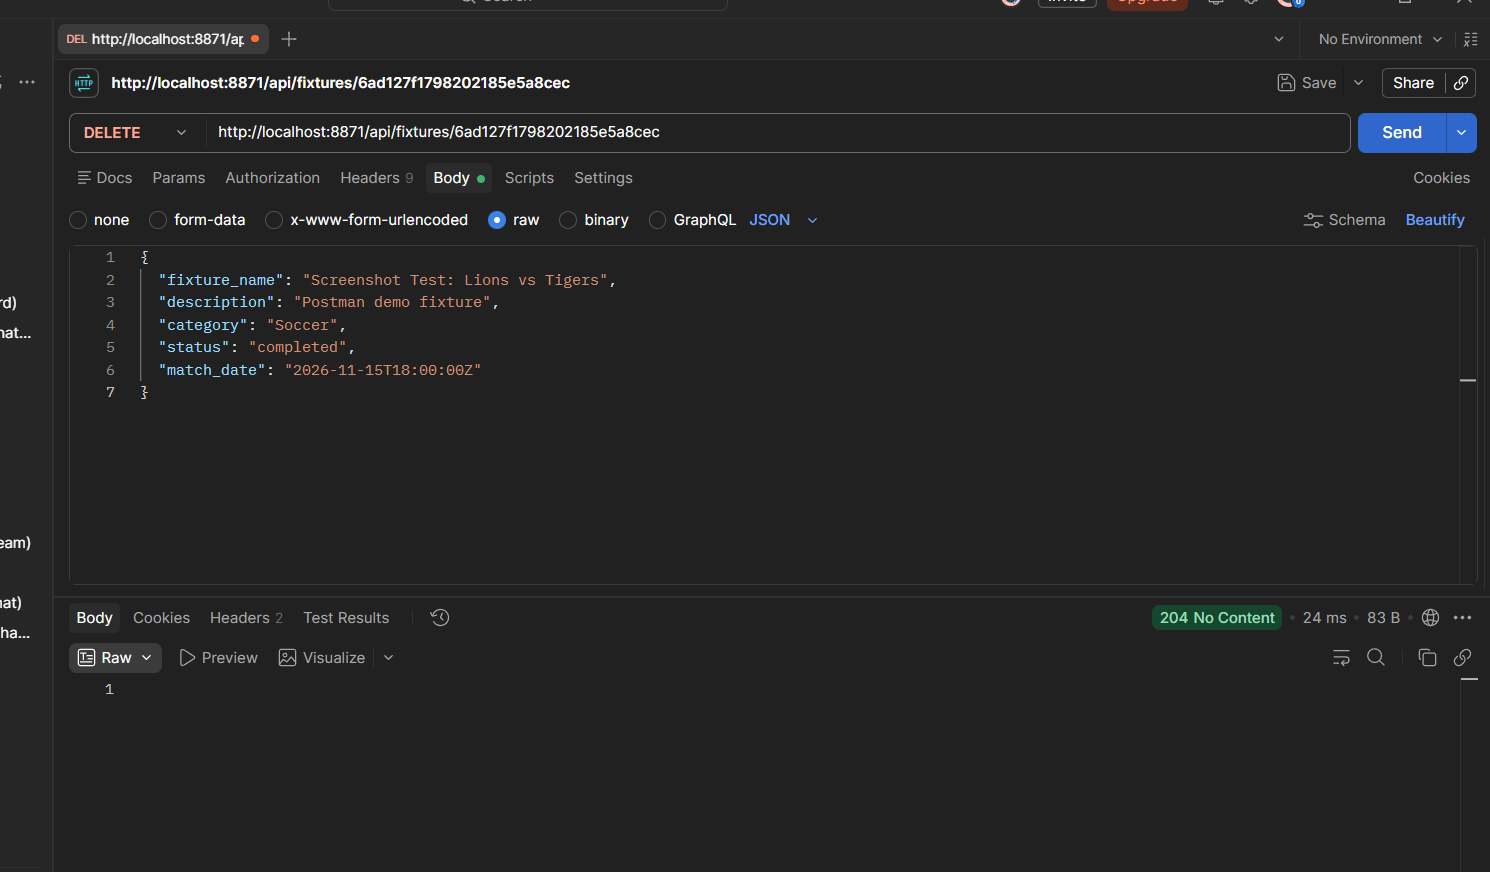
\includegraphics[width=0.80\linewidth,height=0.34\textheight,keepaspectratio]{screenshots/part1_delete.png}\\[2pt]
\small \textit{Figure 7: DELETE /api/fixtures/\{id\}: 204 No Content.}
\end{center}
\subsection*{III. Data validation}
Invalid data (missing field, 101-character name, bad enum, bad date, wrong type, unknown extra field, malformed JSON) returns 422 with a clear per-field message (\verb|main.py| flattens Pydantic's errors into \verb|[{field, message, type}]|).
\begingroup\lstset{basicstyle=\ttfamily\footnotesize}
\begin{lstlisting}
async def validation_handler(request: Request, exc: RequestValidationError):
    """Clear, flat validation errors: [{field, message}] with HTTP 422."""
    errors = [
        {"field": ".".join(str(p) for p in e["loc"] if p != "body") or "body",
         "message": e["msg"], "type": e["type"]}
        for e in exc.errors()
    ]
    return JSONResponse(status_code=422, content={"detail": "validation failed", "errors": errors})
\end{lstlisting}
\endgroup
\begin{center}
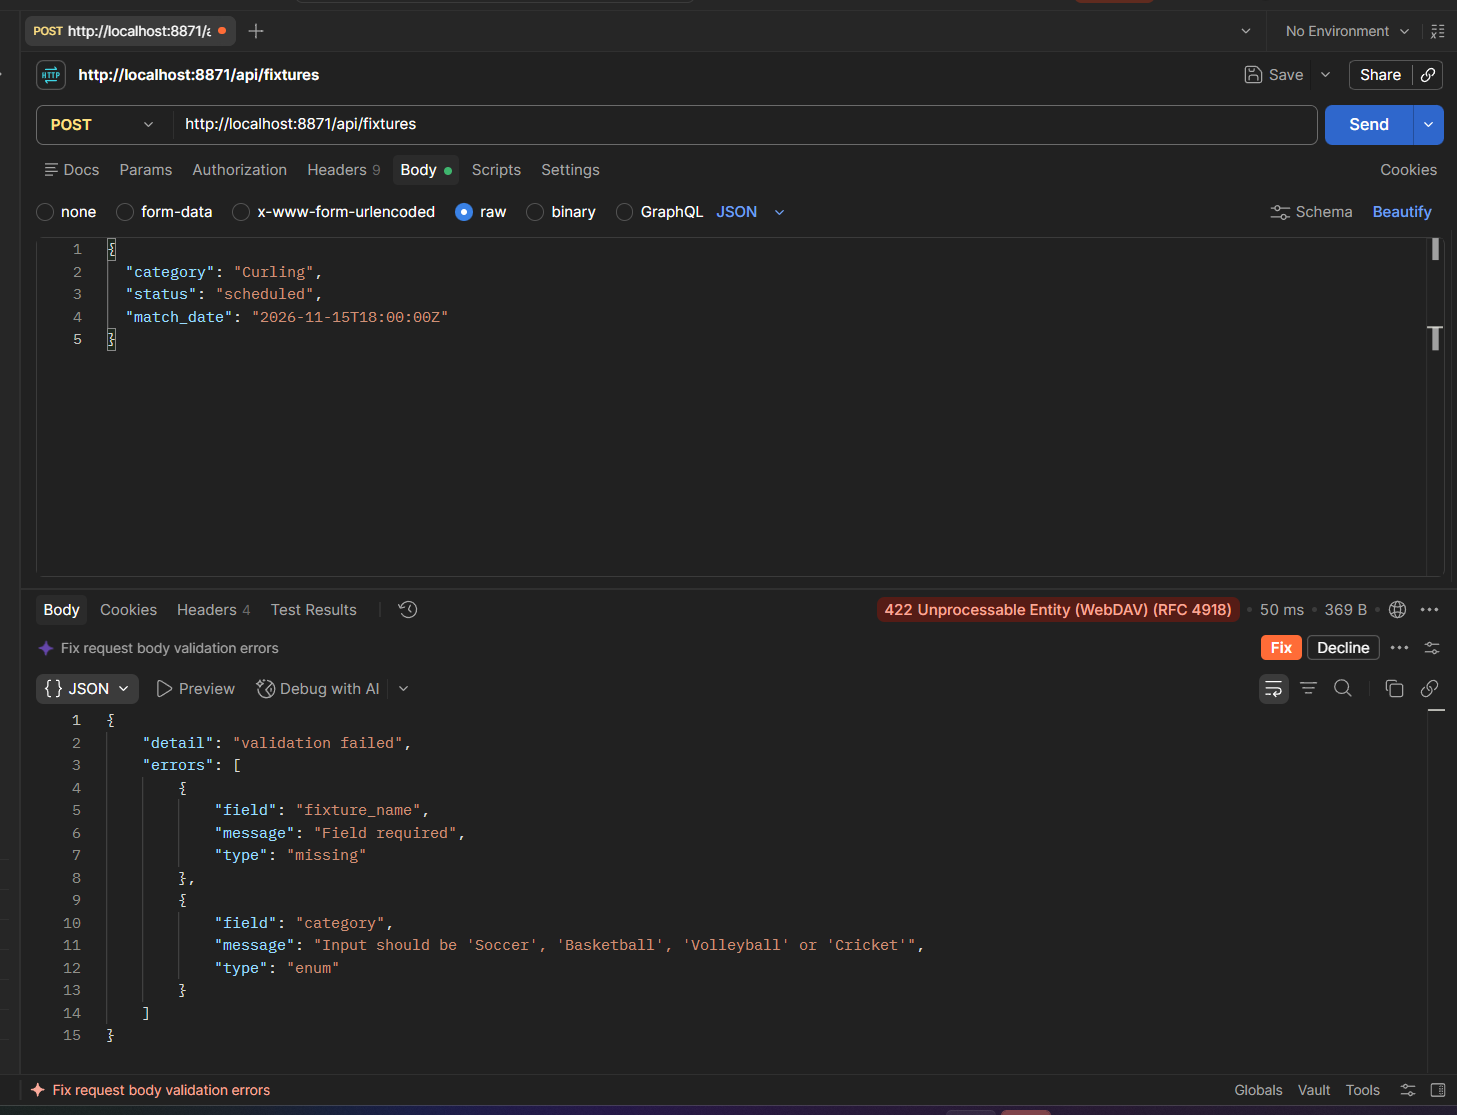
\includegraphics[width=0.80\linewidth,height=0.34\textheight,keepaspectratio]{screenshots/part1_validation_422.png}\\[2pt]
\small \textit{Figure 8: Invalid POST (missing name, category ``Curling''): 422 with per-field errors.}
\end{center}
\begin{center}
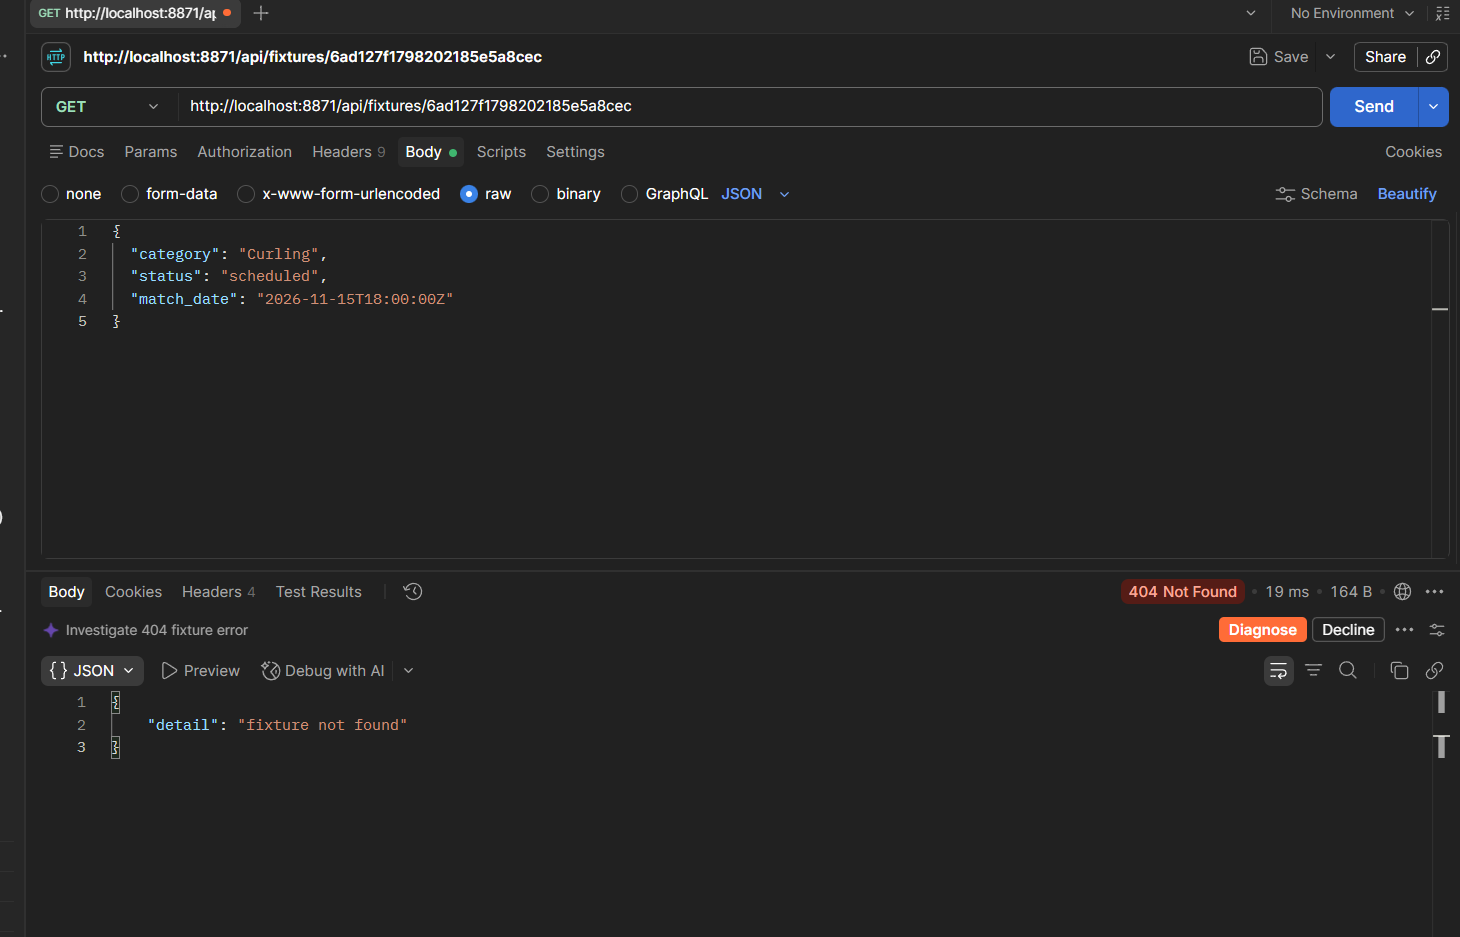
\includegraphics[width=0.80\linewidth,height=0.34\textheight,keepaspectratio]{screenshots/part1_get_404.png}\\[2pt]
\small \textit{Figure 9: GET on the deleted id: 404 ``fixture not found''.}
\end{center}
The live test (\verb|test_part1.py|, real HTTP, then MongoDB checked directly) passed all 26 checks, including a direct insert of a 101-character name being rejected by the database validator itself:
\begingroup\lstset{basicstyle=\ttfamily\scriptsize}
\begin{lstlisting}
[PASS] create returns 201
[PASS] default status is 'scheduled'
[PASS] created_at == updated_at on create
[PASS] list contains created fixture
[PASS] get by id returns 200
[PASS] update returns 200 + new status
[PASS] updated_at advanced
[PASS] POST missing required fixture_name -> 422
[PASS] POST name too long (101 chars) -> 422
[PASS] POST invalid category enum -> 422
[PASS] POST invalid status enum -> 422
[PASS] POST bad date format -> 422
[PASS] POST wrong type (name is a number) -> 422
[PASS] POST unknown extra field -> 422
[PASS] malformed JSON -> 422
[PASS] unknown id -> 404
[PASS] malformed id -> 400
[PASS] PUT unknown id -> 404
[PASS] PUT invalid enum -> 422
[PASS] DB doc persisted with updated status
[PASS] DB stores match_date as BSON date
[PASS] DB validator rejects 101-char name
[PASS] delete returns 204
[PASS] get after delete -> 404
[PASS] second delete -> 404
[PASS] DB doc really gone
26/26 checks passed
\end{lstlisting}
\endgroup
\section*{Part 2 -- Short-, Long-, and Episodic Memory}
Same database \verb|s9871_doc|, new collections \verb|messages|, \verb|summaries|, \verb|episodes| (Part 1's collection is unchanged). Short-term memory is a sliding window of the last \verb|SHORT_TERM_N| messages; long-term memory is a session summary every \verb|SUMMARIZE_EVERY_USER_MSGS| user messages plus a lifetime summary (\verb|scope='user'|, \verb|session_id=null|) condensed from session summaries; episodic memory stores up to 3 facts per user message with an importance score and a 384-float embedding, retrieved by cosine similarity. All model calls go through the HW1 adapter \verb|src/model_client.py|.
\subsection*{Collections}
\begingroup\lstset{basicstyle=\ttfamily\scriptsize}
\begin{lstlisting}
def _init_memory_collections(d) -> None:
    """HW6 Part 2: messages / summaries / episodes (Part 1's collection untouched)."""
    specs = {
        "messages": {
            "required": ["user_id", "session_id", "role", "content", "created_at"],
            "properties": {"role": {"enum": ["user", "assistant"]},
                           "content": {"bsonType": "string"}},
            "indexes": [[("user_id", ASCENDING), ("session_id", ASCENDING), ("created_at", ASCENDING)]],
        },
        "summaries": {
            "required": ["user_id", "session_id", "scope", "text", "created_at"],
            "properties": {"scope": {"enum": ["session", "user"]},
                           "session_id": {"bsonType": ["string", "null"]}},
            "indexes": [[("user_id", ASCENDING), ("scope", ASCENDING), ("created_at", ASCENDING)]],
        },
        "episodes": {
            "required": ["user_id", "session_id", "fact", "importance", "embedding", "created_at"],
            "properties": {"importance": {"bsonType": "double", "minimum": 0, "maximum": 1},
                           "embedding": {"bsonType": "array"}},
            "indexes": [[("user_id", ASCENDING), ("created_at", ASCENDING)]],
        },
    }
    d["usage_log"].create_index([("user_id", ASCENDING), ("ts", ASCENDING)])  # Part 3 cost log (no validator)
    for name, spec in specs.items():
        validator = {"$jsonSchema": {"bsonType": "object", "required": spec["required"],
                                     "properties": spec["properties"]}}
        if name not in d.list_collection_names():
            d.create_collection(name, validator=validator)
        else:
            d.command("collMod", name, validator=validator)
        for idx in spec["indexes"]:
            d[name].create_index(idx)
\end{lstlisting}
\endgroup
\begin{center}
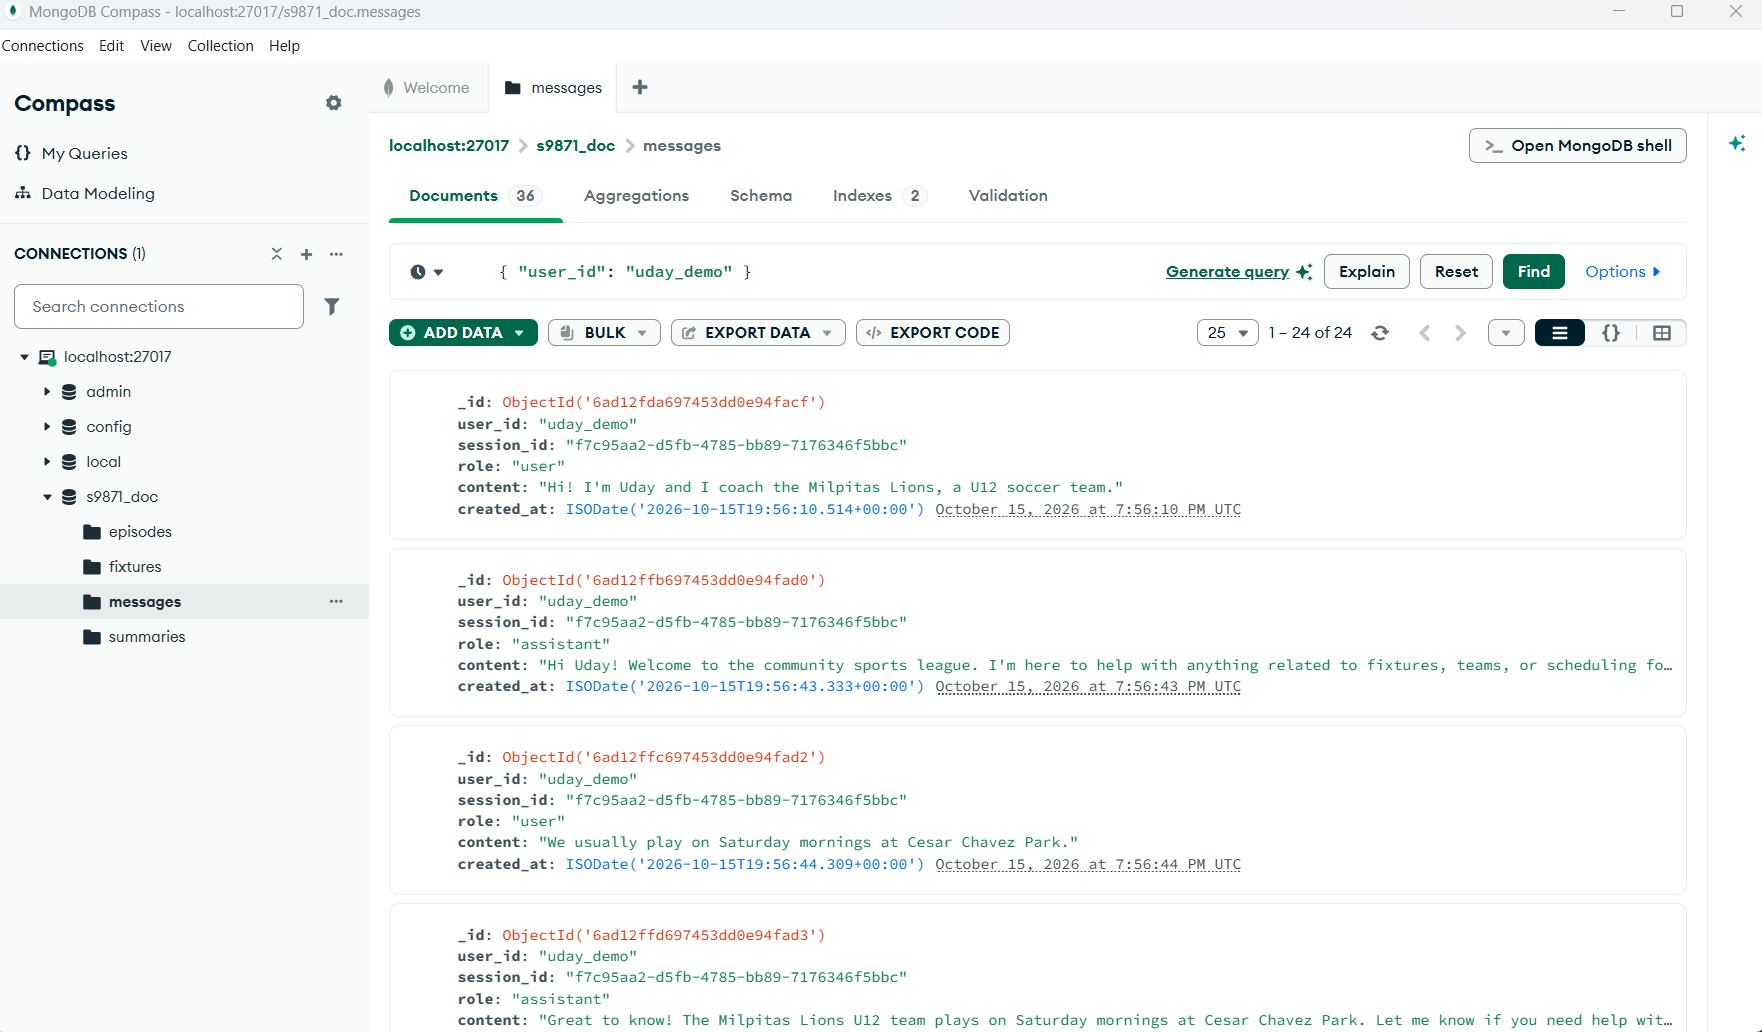
\includegraphics[width=0.80\linewidth,height=0.28\textheight,keepaspectratio]{screenshots/part2_compass_messages.png}\\[2pt]
\small \textit{Figure 10: Compass: \texttt{messages} collection (filter \texttt{user\_id: uday\_demo}), 24 documents.}
\end{center}
\begin{center}
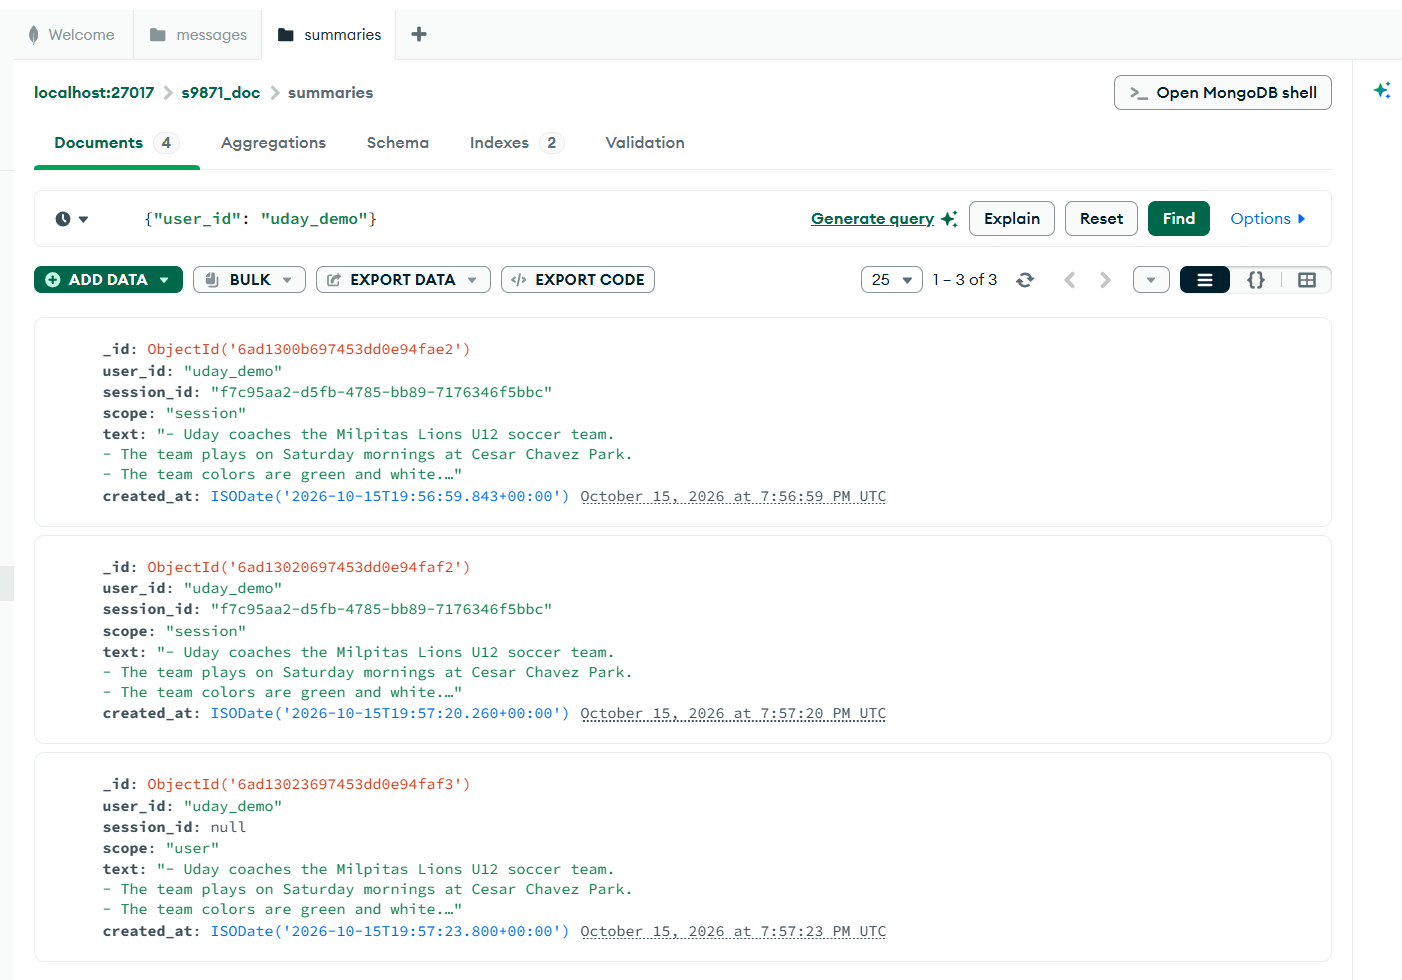
\includegraphics[width=0.80\linewidth,height=0.28\textheight,keepaspectratio]{screenshots/part2_compass_summaries.png}\\[2pt]
\small \textit{Figure 11: Compass: \texttt{summaries} -- two \texttt{scope: session} and one \texttt{scope: user} with \texttt{session\_id: null}.}
\end{center}
\begin{center}
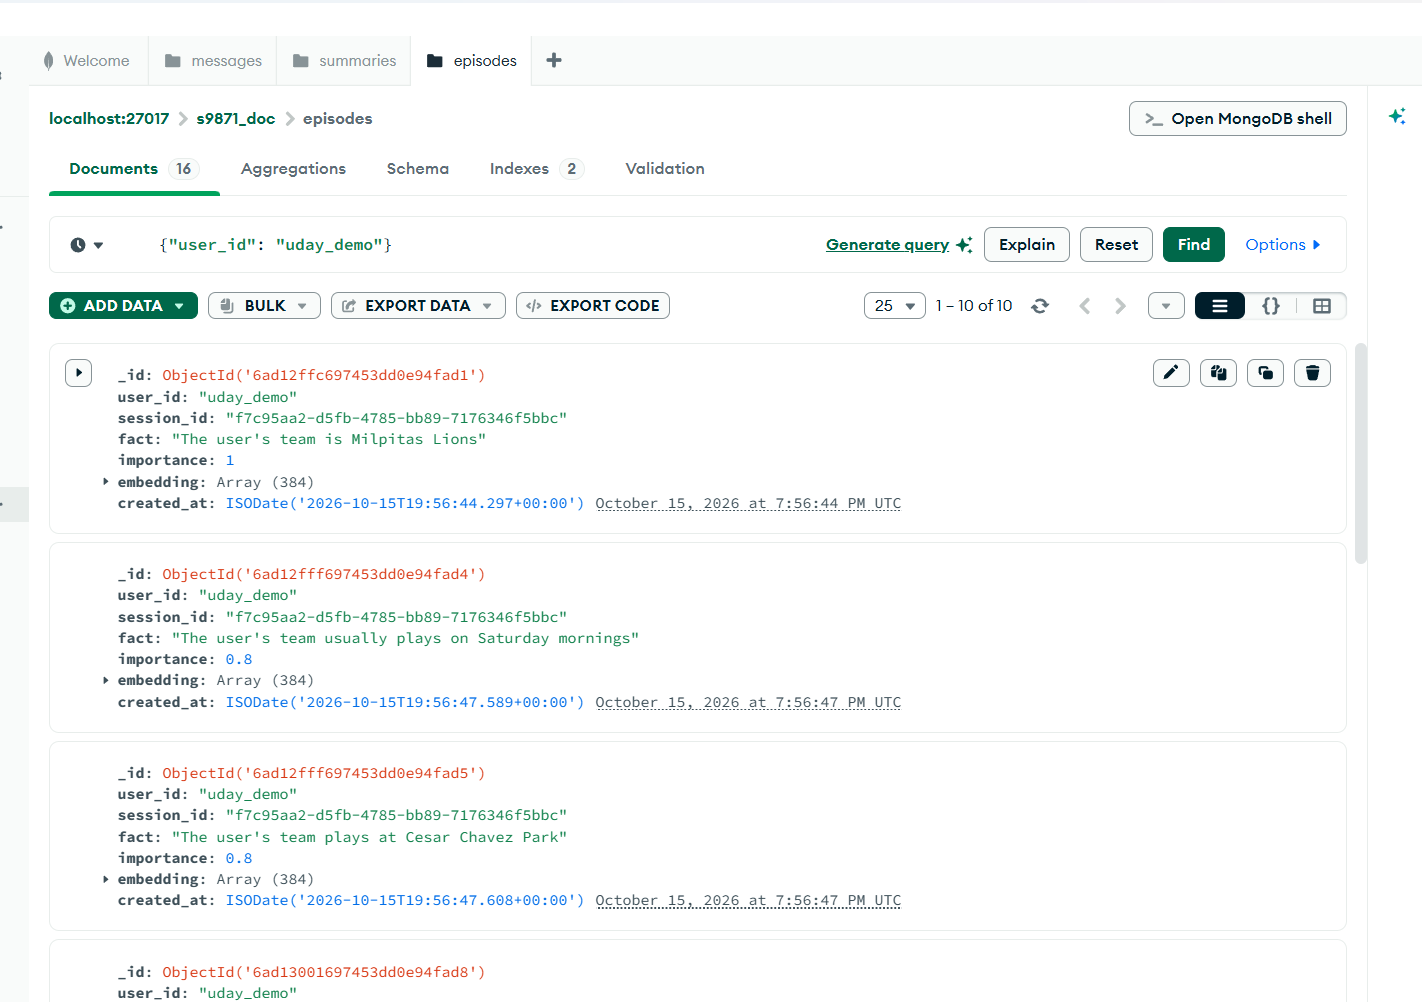
\includegraphics[width=0.80\linewidth,height=0.28\textheight,keepaspectratio]{screenshots/part2_compass_episodes.png}\\[2pt]
\small \textit{Figure 12: Compass: \texttt{episodes} with \texttt{importance} and a 384-element \texttt{embedding} array.}
\end{center}
\subsection*{Short-term memory, summaries and the model adapter}
Short-term memory is a query for the last N messages of the session (oldest first), excluding the message just saved because it is passed to the model separately. The newest summary of each scope is fetched the same way. All model calls go through \verb|llm.complete|, a thin wrapper over the HW1 adapter (\verb|ModelClient|) that adds a lock, token/latency measurement and a per-request call log; the only change to the HW1 adapter was two optional constructor arguments (\verb|reasoning|, \verb|seed|) whose defaults keep earlier homeworks unchanged.
\begingroup\lstset{basicstyle=\ttfamily\scriptsize}
\begin{lstlisting}
def save_message(user_id: str, session_id: str, role: str, content: str) -> dict:
    doc = {"user_id": user_id, "session_id": session_id, "role": role,
           "content": content, "created_at": _now()}
    doc["_id"] = db.get_db()["messages"].insert_one(doc).inserted_id
    return doc

def short_term_window(user_id: str, session_id: str, n: int, before_id=None) -> list[dict]:
    """Last n messages of the session, oldest first. `before_id` excludes the
    message that was just saved (it is passed to the model separately)."""
    query = {"user_id": user_id, "session_id": session_id}
    if before_id is not None:
        query["_id"] = {"$lt": before_id}
    docs = list(db.get_db()["messages"].find(query).sort("_id", -1).limit(max(n, 0)))
    return list(reversed(docs))

def latest_summary(user_id: str, scope: str, session_id: str | None = None) -> dict | None:
    query = {"user_id": user_id, "scope": scope}
    if scope == "session" and session_id is not None:
        query["session_id"] = session_id
    return db.get_db()["summaries"].find_one(query, sort=[("created_at", -1), ("_id", -1)])

def count_user_messages(user_id: str, session_id: str) -> int:
    return db.get_db()["messages"].count_documents(
        {"user_id": user_id, "session_id": session_id, "role": "user"})
\end{lstlisting}
\endgroup
\begingroup\lstset{basicstyle=\ttfamily\scriptsize}
\begin{lstlisting}
def complete(messages: list[dict]) -> dict:
    """Run one completion. Returns {text, prompt_tokens, completion_tokens, latency_ms}."""
    with _lock:
        client = _get_client()
        client.history = []
        before_in, before_out = client.cumulative_input_tokens, client.cumulative_output_tokens
        t0 = time.perf_counter()
        try:
            text = client.complete(messages)
        except Exception as exc:  # connection refused, model missing, ...
            raise LLMError(f"model call failed: {exc}") from exc
        latency_ms = (time.perf_counter() - t0) * 1000
        result = {
            "text": (text or "").strip(),
            "prompt_tokens": client.cumulative_input_tokens - before_in,
            "completion_tokens": client.cumulative_output_tokens - before_out,
            "latency_ms": round(latency_ms, 1),
        }
    calls = getattr(_local, "calls", None)
    if calls is not None:
        calls.append({k: v for k, v in result.items() if k != "text"})
    return result

def start_tracking() -> None:
    """Begin recording every complete() call made on this thread (one request)."""
    _local.calls = []

def stop_tracking() -> list[dict]:
    calls, _local.calls = getattr(_local, "calls", []), None
    return calls
\end{lstlisting}
\endgroup
\begingroup\lstset{basicstyle=\ttfamily\scriptsize}
\begin{lstlisting}
def __init__(self, model="qwen3:8b", temperature=0.7, reasoning=None, seed=None):
        # HW6: `reasoning=False` turns off qwen3's hidden thinking phase
        # (Ollama think=False). Default None keeps the earlier homeworks'
        # behaviour unchanged.
        extra = {} if reasoning is None else {"reasoning": reasoning}
        if seed is not None:  # HW6 Part 3: reproducible runs (SEED from CLAUDE.md)
            extra["seed"] = seed
        self._llm = ChatOllama(model=model, temperature=temperature, **extra)
        self.history = []  # list of {"role": ..., "content": ...} dicts

        self.turn_count = 0
        self.cumulative_input_tokens = 0
        self.cumulative_output_tokens = 0
\end{lstlisting}
\endgroup
\subsection*{Endpoints}
The request model rejects empty messages, bad user ids and unknown fields (all return 422):
\begingroup\lstset{basicstyle=\ttfamily\scriptsize}
\begin{lstlisting}
USER_ID_PATTERN = r"^[A-Za-z0-9_.@-]{1,64}$"

class ChatRequest(BaseModel):
    model_config = ConfigDict(extra="forbid")
    user_id: str = Field(..., pattern=USER_ID_PATTERN)
    session_id: str | None = Field(None, min_length=1, max_length=64)
    message: str = Field(..., min_length=1, max_length=4000)
    # Part 3 probes: answer using memory but write nothing (no messages, episodes
    # or summaries), so one probe cannot leak into the next.
    read_only: bool = False
\end{lstlisting}
\endgroup
\texttt{POST /api/chat} (the parts after the memory pipeline that only record Part 3's cost data are included too):
\begingroup\lstset{basicstyle=\ttfamily\scriptsize}
\begin{lstlisting}
def chat(req: ChatRequest):
    t_request = time.perf_counter()
    session_id = req.session_id or str(uuid.uuid4())
    window_n, summarize_every = config.effective_memory_params()
    top_k = config.settings["EPISODE_TOP_K"]
    llm.start_tracking()
    try:
        saved = None if req.read_only else memory.save_message(
            req.user_id, session_id, "user", req.message)
        window = memory.short_term_window(req.user_id, session_id, window_n,
                                          before_id=saved["_id"] if saved else None)
        sess = memory.latest_summary(req.user_id, "session", session_id)
        life = memory.latest_summary(req.user_id, "user")
        episodes = memory.retrieve_episodes(req.user_id, req.message, top_k)

        messages, parts = memory.build_prompt(
            window, sess["text"] if sess else None, life["text"] if life else None,
            episodes, req.message)
        result = llm.complete(messages)
        reply = result["text"] or "(the model returned an empty reply)"
        new_facts, summaries = [], {"session_summary": None, "lifetime_summary": None}
        if not req.read_only:
            memory.save_message(req.user_id, session_id, "assistant", reply)
            new_facts = memory.extract_and_store_episodes(req.user_id, session_id, req.message)
            summaries = memory.maybe_summarize(req.user_id, session_id, every=summarize_every)
    except llm.LLMError as exc:
        llm.stop_tracking()
        raise HTTPException(status_code=502, detail=str(exc))
    calls = llm.stop_tracking()
    request_ms = round((time.perf_counter() - t_request) * 1000, 1)

    # ---- Part 3: per-request memory-cost record
    comp = {name: tokens.count(text) for name, text in parts.items()}
    prompt_tokens_sum = (comp["system_primer"] + comp["long_term_summary"]
                         + comp["short_term_window"] + comp["episodic_facts"]
                         + comp["current_message"])
    usage = {
        "prompt_tokens": result["prompt_tokens"],
        "completion_tokens": result["completion_tokens"],
        "latency_ms": result["latency_ms"],
        "request_latency_ms": request_ms,
        "llm_calls": len(calls),
        "total_prompt_tokens": sum(c["prompt_tokens"] for c in calls),
        "total_completion_tokens": sum(c["completion_tokens"] for c in calls),
        "component_tokens": {**comp, "template_overhead": result["prompt_tokens"] - prompt_tokens_sum},
    }
    db.get_db()["usage_log"].insert_one({
        "ts": datetime.now(timezone.utc), "user_id": req.user_id, "session_id": session_id,
        "read_only": req.read_only,
        "user_msg_count": memory.count_user_messages(req.user_id, session_id),
        "settings": {**config.settings, "window_n": window_n, "summarize_every": summarize_every},
        **usage,
    })

    return {
        "reply": reply,
        "user_id": req.user_id,
        "session_id": session_id,
        "memory_used": {
            "short_term_count": len(window),
            "short_term_messages": [{"role": m["role"], "content": m["content"]} for m in window],
            "session_summary": sess["text"] if sess else None,
            "long_term_summary": life["text"] if life else None,
            "episodic_facts": episodes,
        },
        "memory_written": {
            "new_episodes": new_facts,
            "session_summary_created": summaries["session_summary"] is not None,
            "lifetime_summary_created": summaries["lifetime_summary"] is not None,
        },
        "usage": usage,
        "prompt_parts": parts,
    }
\end{lstlisting}
\endgroup
\texttt{GET /api/memory/\{user\_id\}} and \texttt{GET /api/aggregate/\{user\_id\}}:
\begingroup\lstset{basicstyle=\ttfamily\scriptsize}
\begin{lstlisting}
def get_memory(user_id: str):
    d = db.get_db()
    msgs = list(d["messages"].find({"user_id": user_id}).sort("_id", -1).limit(16))[::-1]
    eps = list(d["episodes"].find({"user_id": user_id}).sort("_id", -1).limit(20))
    sess = memory.latest_summary(user_id, "session")
    life = memory.latest_summary(user_id, "user")
    if not msgs and not eps and not sess and not life:
        raise HTTPException(status_code=404, detail=f"no memory stored for user '{user_id}'")
    return {
        "user_id": user_id,
        "messages": [_iso(m, "session_id", "role", "content", "created_at") for m in msgs],
        "latest_session_summary": _iso(sess, "session_id", "text", "created_at") if sess else None,
        "latest_lifetime_summary": _iso(life, "text", "created_at") if life else None,
        "episodes": [{**_iso(e, "session_id", "fact", "importance", "created_at"),
                      "embedding_dim": len(e.get("embedding", []))} for e in eps],
    }

def aggregate(user_id: str):
    d = db.get_db()
    daily = d["messages"].aggregate([
        {"$match": {"user_id": user_id}},
        {"$group": {"_id": {"$dateToString": {"format": "%Y-%m-%d", "date": "$created_at"}},
                    "count": {"$sum": 1}}},
        {"$sort": {"_id": 1}},
    ])
    recent = d["summaries"].find({"user_id": user_id}).sort("created_at", -1).limit(5)
    return {
        "user_id": user_id,
        "daily_message_counts": [{"date": r["_id"], "count": r["count"]} for r in daily],
        "recent_summaries": [_iso(s, "scope", "session_id", "text", "created_at") for s in recent],
    }
\end{lstlisting}
\endgroup
\subsection*{Memory logic}
Episode extraction (the model returns facts, the code parses and embeds them), embedding and cosine retrieval, the summarisation trigger, and prompt assembly:
\begingroup\lstset{basicstyle=\ttfamily\scriptsize}
\begin{lstlisting}
SYSTEM_PRIMER = (
    "You are a friendly assistant for a community sports league. You help with "
    "fixtures, teams and scheduling questions. Use the remembered context below "
    "when it is relevant, never invent facts about the user, and keep replies "
    "short (1-3 sentences)."
)

_EXTRACT_PROMPT = (
    "Extract up to {max_facts} short, durable facts about the USER from the message "
    "below (preferences, their own team, schedules, constraints, personal details). "
    "Rules: 'we/our/my team' refers to the user's own team; a team the user calls a "
    "rival or opponent is NOT the user's team - state it as 'The user's rival/opponent "
    "is X'. Use only what the message says. Ignore greetings and questions with no "
    "facts. Reply with ONLY a JSON array like "
    '[{{"fact": "short sentence", "importance": 0.0-1.0}}]. Reply [] if there are none.'
    "\n\nMessage: {message}"
)

def parse_facts(raw: str, max_facts: int) -> list[dict]:
    """Defensive parse of the model's JSON array; returns [] on anything odd."""
    match = re.search(r"\[.*\]", raw, flags=re.S)
    if not match:
        return []
    try:
        items = json.loads(match.group(0))
    except json.JSONDecodeError:
        return []
    facts = []
    for it in items if isinstance(items, list) else []:
        if not isinstance(it, dict):
            continue
        fact = str(it.get("fact", "")).strip()
        try:
            importance = float(it.get("importance", 0.5))
        except (TypeError, ValueError):
            importance = 0.5
        if fact:
            facts.append({"fact": fact[:200], "importance": min(1.0, max(0.0, importance))})
    return facts[:max_facts]

def extract_and_store_episodes(user_id: str, session_id: str, message: str) -> list[dict]:
    res = llm.complete([{"role": "user", "content": _EXTRACT_PROMPT.format(
        max_facts=config.settings["MAX_FACTS_PER_MESSAGE"], message=message)}])
    facts = parse_facts(res["text"], config.settings["MAX_FACTS_PER_MESSAGE"])
    stored = []
    for f in facts:
        doc = {"user_id": user_id, "session_id": session_id, "fact": f["fact"],
               "importance": f["importance"], "embedding": embeddings.embed(f["fact"]),
               "created_at": _now()}
        db.get_db()["episodes"].insert_one(doc)
        stored.append({"fact": doc["fact"], "importance": doc["importance"]})
    return stored

def retrieve_episodes(user_id: str, query_text: str, k: int) -> list[dict]:
    """Top-k stored facts for this user by cosine similarity to the query."""
    candidates = list(db.get_db()["episodes"].find({"user_id": user_id}))
    top = embeddings.cosine_top_k(embeddings.embed(query_text), candidates, k)
    return [{"fact": e["fact"], "importance": e["importance"],
             "score": round(e["score"], 4), "session_id": e["session_id"]} for e in top]
\end{lstlisting}
\endgroup
\begingroup\lstset{basicstyle=\ttfamily\scriptsize}
\begin{lstlisting}
def embed(text: str) -> list[float]:
    """Return a unit-length embedding as a plain list of floats (BSON-safe)."""
    vec = _get_model().encode(text, normalize_embeddings=True)
    return [float(x) for x in np.asarray(vec)]

def cosine_top_k(query_vec: list[float], candidates: list[dict], k: int) -> list[dict]:
    """Rank candidate episode docs by cosine similarity to query_vec.
    Vectors are unit length, so cosine == dot product. Adds a `score` key."""
    if not candidates or k <= 0:
        return []
    q = np.asarray(query_vec, dtype=np.float32)
    mat = np.asarray([c["embedding"] for c in candidates], dtype=np.float32)
    denom = (np.linalg.norm(mat, axis=1) * np.linalg.norm(q)) + 1e-9
    scores = (mat @ q) / denom
    order = np.argsort(-scores)[:k]
    return [{**candidates[i], "score": float(scores[i])} for i in order]
\end{lstlisting}
\endgroup
Summaries: every M user messages a session summary is written (bullets only, updating the previous one), and every second session summary is condensed into the lifetime summary. \verb|clean_bullets| drops model commentary.
\begingroup\lstset{basicstyle=\ttfamily\scriptsize}
\begin{lstlisting}
def clean_bullets(text: str) -> str:
    """Keep only bullet lines (drops model commentary such as a trailing
    '(No additional information...)'); falls back to the raw text."""
    lines = [ln.rstrip() for ln in text.splitlines()
             if ln.strip().startswith(("-", "*", "\u2022"))]
    return "\n".join(lines) if lines else text.strip()

def maybe_summarize(user_id: str, session_id: str, every: int | None = None) -> dict:
    """Every SUMMARIZE_EVERY_USER_MSGS user messages: write a session summary
    (scope='session'); every LIFETIME_EVERY_N_SESSION_SUMMARIES session summaries,
    condense into the lifetime summary (scope='user', session_id=None)."""
    every = config.effective_memory_params()[1] if every is None else every
    n_user = count_user_messages(user_id, session_id)
    out = {"session_summary": None, "lifetime_summary": None}
    if every <= 0 or n_user == 0 or n_user % every != 0:
        return out

    col = db.get_db()["messages"]
    recent = list(col.find({"user_id": user_id, "session_id": session_id})
                  .sort("_id", -1).limit(every * 2))[::-1]
    prev = latest_summary(user_id, "session", session_id)
    prompt = ("Summarize the conversation below into at most 5 concise bullet points "
              "capturing facts about the user and decisions made. Output ONLY the bullet "
              "list, each line starting with '- ', with no other commentary. "
              + (f"Previous summary (update it: keep facts that are still true AND add every "
                 f"new fact from the conversation below):\n{prev['text']}\n\n" if prev else "")
              + f"Conversation:\n{_transcript(recent)}")
    text = clean_bullets(llm.complete([{"role": "user", "content": prompt}])["text"])
    if not text:
        return out
    db.get_db()["summaries"].insert_one({
        "user_id": user_id, "session_id": session_id, "scope": "session",
        "text": text, "created_at": _now()})
    out["session_summary"] = text

    n_sess = db.get_db()["summaries"].count_documents({"user_id": user_id, "scope": "session"})
    if n_sess % config.settings["LIFETIME_EVERY_N_SESSION_SUMMARIES"] == 0:
        sess = list(db.get_db()["summaries"].find({"user_id": user_id, "scope": "session"})
                    .sort("created_at", -1).limit(4))[::-1]
        old = latest_summary(user_id, "user")
        prompt = ("Merge these notes about one user into at most 6 concise bullet points. "
                  "Keep durable facts, drop one-off details, and prefer the newest "
                  "information if two notes conflict. Output ONLY the bullet list, each line "
                  "starting with '- ', with no other commentary.\n\n"
                  + (f"Existing lifetime summary:\n{old['text']}\n\n" if old else "")
                  + "Session summaries:\n" + "\n---\n".join(s["text"] for s in sess))
        life = clean_bullets(llm.complete([{"role": "user", "content": prompt}])["text"])
        if life:
            db.get_db()["summaries"].insert_one({
                "user_id": user_id, "session_id": None, "scope": "user",
                "text": life, "created_at": _now()})
            out["lifetime_summary"] = life
    return out
\end{lstlisting}
\endgroup
Prompt assembly (system primer + long-term summaries, short-term window, current message, then episodic facts); each component is also returned separately so Part 3 can count its tokens:
\begingroup\lstset{basicstyle=\ttfamily\scriptsize}
\begin{lstlisting}
def build_prompt(window: list[dict], session_summary: str | None,
                 lifetime_summary: str | None, episodes: list[dict],
                 message: str) -> tuple[list[dict], dict]:
    """Order: system primer + long-term summaries, short-term window, current
    message, episodic facts. Returns (messages, parts) - `parts` keeps each
    component's text separate so Part 3 can attribute tokens per component."""
    long_term = ""
    if lifetime_summary:
        long_term += f"\n\nLifetime summary of this user:\n{lifetime_summary}"
    if session_summary:
        long_term += f"\n\nSummary of this session so far:\n{session_summary}"
    episodic = ""
    if episodes:
        episodic = ("\n\nRelevant remembered facts about the user:\n"
                    + "\n".join(f"- {e['fact']}" for e in episodes))

    messages = [{"role": "system", "content": SYSTEM_PRIMER + long_term}]
    messages += [{"role": m["role"], "content": m["content"]} for m in window]
    messages.append({"role": "user", "content": message + episodic})
    parts = {
        "system_primer": SYSTEM_PRIMER,
        "long_term_summary": long_term.strip(),
        "short_term_window": "\n".join(f"{m['role']}: {m['content']}" for m in window),
        "episodic_facts": episodic.strip(),
        "current_message": message,
    }
    return messages, parts
\end{lstlisting}
\endgroup
\subsection*{Running it: 12-message conversation}
\begin{center}
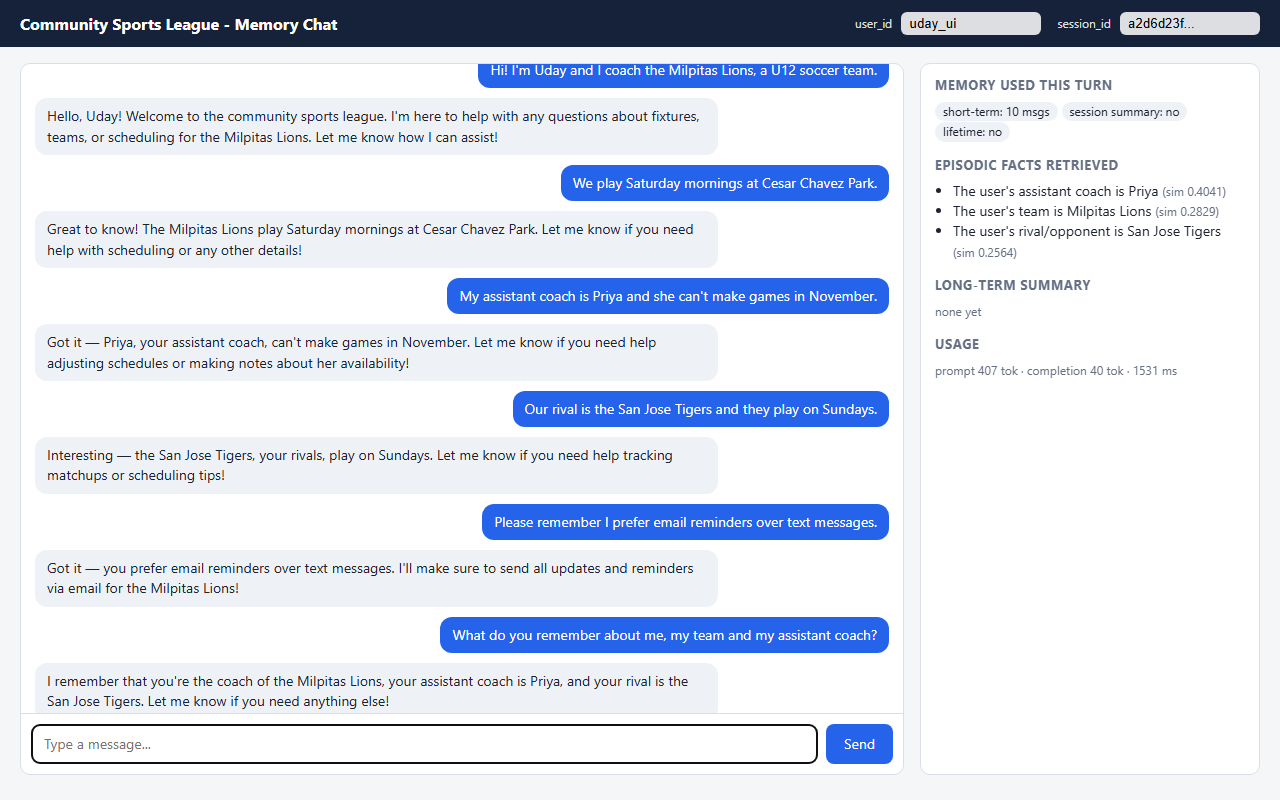
\includegraphics[width=0.80\linewidth,height=0.34\textheight,keepaspectratio]{screenshots/part2_chat_ui.png}\\[2pt]
\small \textit{Figure 13: Mini chat page (\texttt{/chat}) driven by Playwright: 6 messages, replies, and the memory used for the last turn (10 short-term messages, 3 episodic facts with similarity scores).}
\end{center}
\texttt{GET /api/memory/uday\_demo} (trimmed for length; the full 16-message JSON is in \url{raw/part2_memory_uday_demo.json}):
\begingroup\lstset{basicstyle=\ttfamily\scriptsize}
\begin{lstlisting}
{
 "user_id": "uday_demo",
 "messages": "<16 messages, first shown>",
 "first_message": {
  "session_id": "f7c95aa2-d5fb-4785-bb89-7176346f5bbc",
  "role": "user",
  "content": "My assistant coach is Priya and she can't make games in November.",
  "created_at": "2026-10-15T19:56:51.514000+00:00"
 },
 "latest_session_summary": {
  "session_id": "f7c95aa2-d5fb-4785-bb89-7176346f5bbc",
  "text": "- Uday coaches the Milpitas Lions U12 soccer team.\n- The team plays on Saturday mornings at Cesar Chavez Park.\n- The team colors are green and white.\n- Priya, the assistant coach, cannot attend games in November.\n- No peanut snacks are allowed at team events due to Uday's peanut allergy.\n- The next fixture is on November 1st at 6pm against the San Jose Tigers.\n- Email reminders are preferred over text messages.\n- The San Jose Tigers are the main rival, playing on Sundays.",
  "created_at": "2026-10-15T19:57:20.260000+00:00"
 },
 "latest_lifetime_summary": {
  "text": "- Uday coaches the Milpitas Lions U12 soccer team.\n- The team plays on Saturday mornings at Cesar Chavez Park.\n- The team colors are green and white.\n- Priya, the assistant coach, cannot attend games in November.\n- No peanut snacks are allowed at team events due to Uday's peanut allergy.\n- The next fixture is on November 1st at 6pm against the San Jose Tigers.",
  "created_at": "2026-10-15T19:57:23.800000+00:00"
 },
 "episodes": "<10 episodes, first 3 shown>",
 "first_3_episodes": [
  {
   "session_id": "f7c95aa2-d5fb-4785-bb89-7176346f5bbc",
   "fact": "The user prefers email reminders over text messages",
   "importance": 1.0,
   "created_at": "2026-10-15T19:57:13.018000+00:00",
   "embedding_dim": 384
  },
  {
   "session_id": "f7c95aa2-d5fb-4785-bb89-7176346f5bbc",
   "fact": "The user's team is playing against the Tigers on November 1st at 6pm",
   "importance": 0.8,
   "created_at": "2026-10-15T19:57:08.284000+00:00",
   "embedding_dim": 384
  },
  {
   "session_id": "f7c95aa2-d5fb-4785-bb89-7176346f5bbc",
   "fact": "The user's rival/opponent is San Jose Tigers",
   "importance": 1.0,
   "created_at": "2026-10-15T19:57:05.064000+00:00",
   "embedding_dim": 384
  }
 ]
}
\end{lstlisting}
\endgroup
\begin{center}
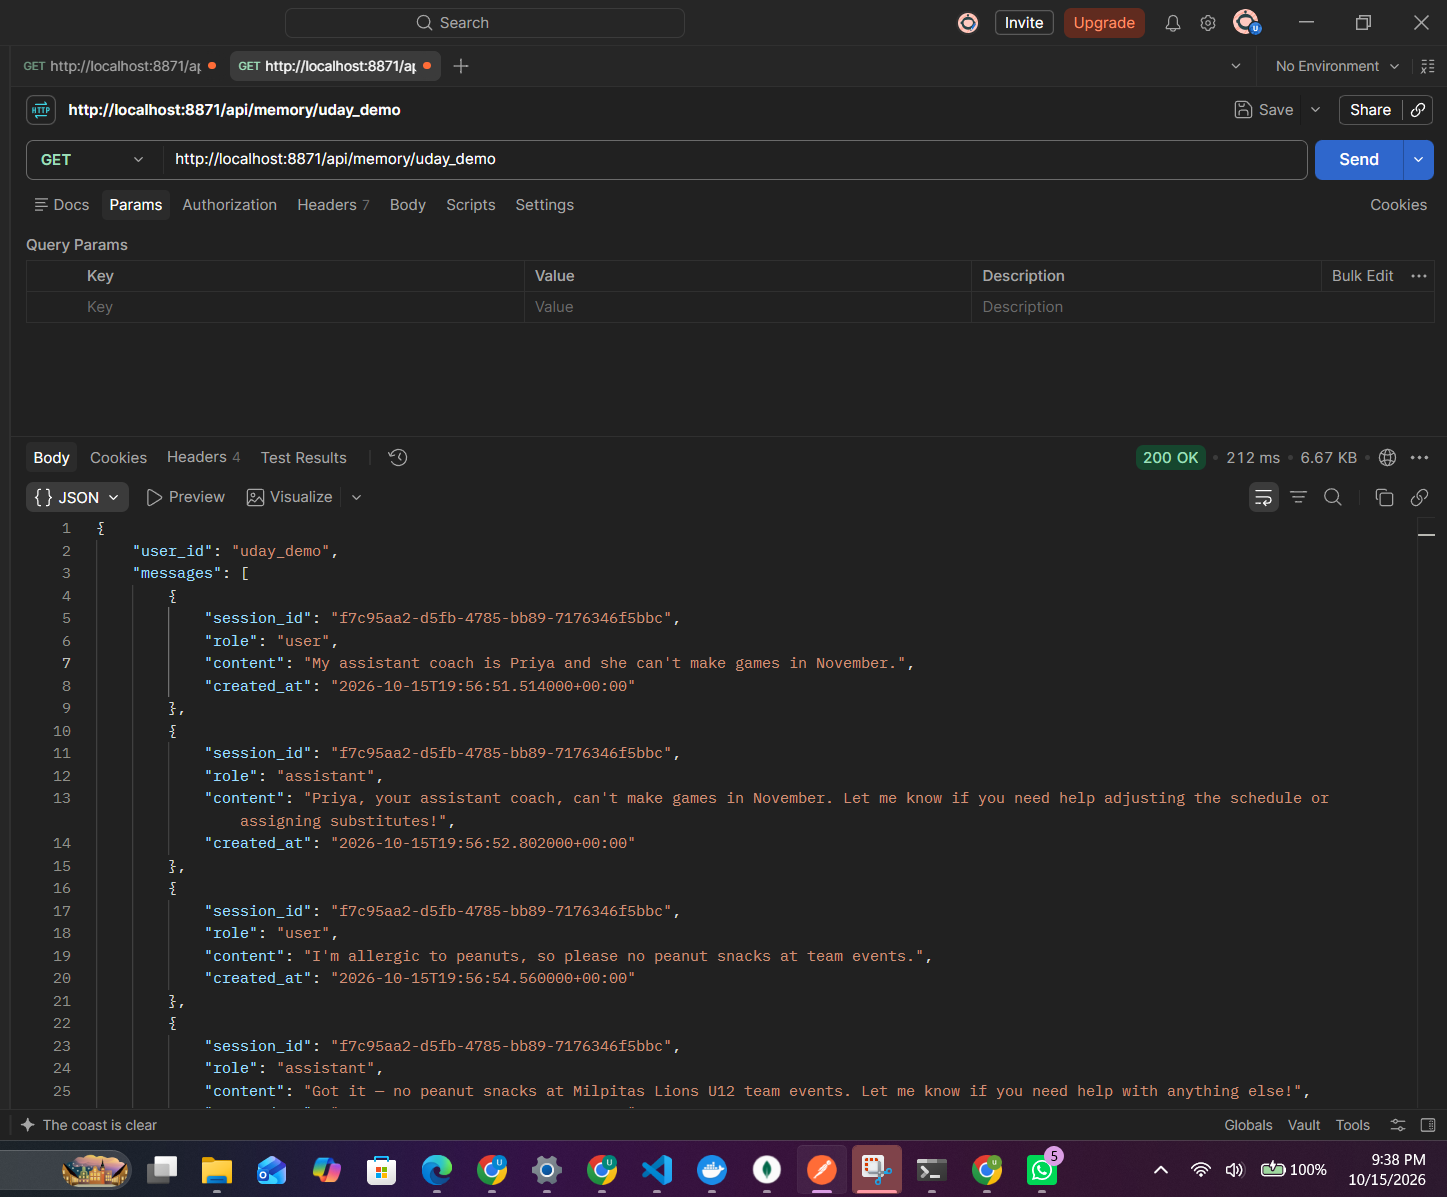
\includegraphics[width=0.80\linewidth,height=0.34\textheight,keepaspectratio]{screenshots/part2_get_memory.png}\\[2pt]
\small \textit{Figure 14: Postman: GET /api/memory/uday\_demo -- 200 OK (top of the JSON; full response in the raw file).}
\end{center}
\texttt{GET /api/aggregate/uday\_demo}:
\begingroup\lstset{basicstyle=\ttfamily\footnotesize}
\begin{lstlisting}
{
 "user_id": "uday_demo",
 "daily_message_counts": [
  {
   "date": "2026-10-15",
   "count": 24
  }
 ],
 "recent_summaries": "<3 summaries: lifetime first, then session summaries>"
}
\end{lstlisting}
\endgroup
\begin{center}
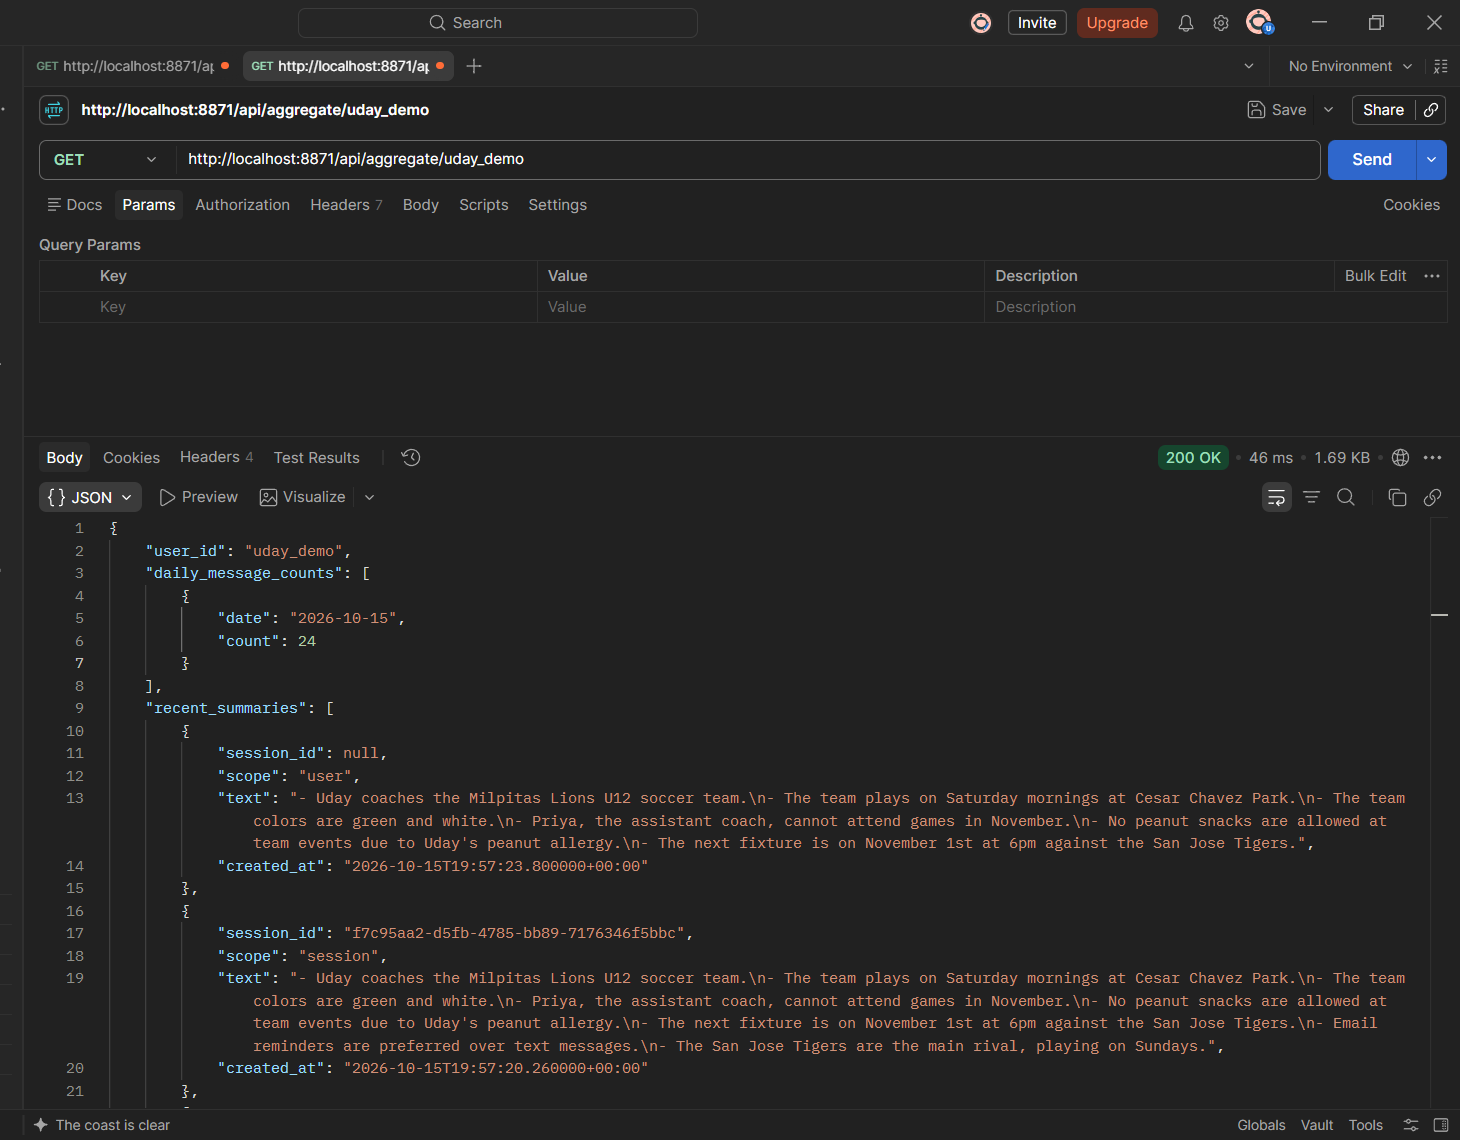
\includegraphics[width=0.80\linewidth,height=0.34\textheight,keepaspectratio]{screenshots/part2_get_aggregate.png}\\[2pt]
\small \textit{Figure 15: Postman: GET /api/aggregate/uday\_demo -- daily counts and the most recent summaries (dates are UTC).}
\end{center}
Two bugs were found by reading the transcripts of a run that had passed all 17 checks, and fixed: the extractor stored ``the user's team is the San Jose Tigers'' (they were the rival), and a leaked model comment ended the lifetime summary. After the prompt fixes the same conversation stored ``the user's rival/opponent is San Jose Tigers'' and the final recall was correct (\verb|RUN_LOG.txt|, runs 1--3).
\section*{Part 3 -- What Memory Costs}
\subsection*{1. Logging memory usage}
Every \verb|/api/chat| request writes one row to a \verb|usage_log| collection (and returns it): prompt and completion tokens of the reply call and of all model calls in the request, tokens per prompt component (counted with the Qwen3 tokenizer; the remainder is reported as chat-template overhead), and latency. Raw results: \verb|raw/part3_turns.csv| (360 rows).
Ollama only reports one prompt-token total per call, so each component's text is counted with the Qwen3 tokenizer and the remainder is the chat-template overhead:
\begingroup\lstset{basicstyle=\ttfamily\scriptsize}
\begin{lstlisting}
def count(text: str) -> int:
    global _tok
    if not text:
        return 0
    with _lock:
        if _tok is None:
            from transformers import AutoTokenizer
            _tok = AutoTokenizer.from_pretrained(config.TOKENIZER_NAME)
    return len(_tok.encode(text))
\end{lstlisting}
\endgroup
\begingroup\lstset{basicstyle=\ttfamily\scriptsize}
\begin{lstlisting}
# ---- Part 3: per-request memory-cost record
comp = {name: tokens.count(text) for name, text in parts.items()}
prompt_tokens_sum = (comp["system_primer"] + comp["long_term_summary"]
                     + comp["short_term_window"] + comp["episodic_facts"]
                     + comp["current_message"])
usage = {
    "prompt_tokens": result["prompt_tokens"],
    "completion_tokens": result["completion_tokens"],
    "latency_ms": result["latency_ms"],
    "request_latency_ms": request_ms,
    "llm_calls": len(calls),
    "total_prompt_tokens": sum(c["prompt_tokens"] for c in calls),
    "total_completion_tokens": sum(c["completion_tokens"] for c in calls),
    "component_tokens": {**comp, "template_overhead": result["prompt_tokens"] - prompt_tokens_sum},
}
db.get_db()["usage_log"].insert_one({
    "ts": datetime.now(timezone.utc), "user_id": req.user_id, "session_id": session_id,
    "read_only": req.read_only,
    "user_msg_count": memory.count_user_messages(req.user_id, session_id),
    "settings": {**config.settings, "window_n": window_n, "summarize_every": summarize_every},
    **usage,
})
\end{lstlisting}
\endgroup
\begingroup\lstset{basicstyle=\ttfamily\scriptsize}
\begin{lstlisting}
turn,reply_prompt_tokens,reply_completion_tokens,total_prompt_tokens,tok_system_primer,tok_long_term_summary,tok_short_term_window,tok_episodic_facts,request_latency_ms
1,101,47,277,48,0,0,0,4131.5
2,215,41,372,48,0,82,45,2678.2
3,280,30,432,48,0,139,52,2160.0
4,247,34,408,48,0,98,51,3034.1
... (first 4 of 360 rows)
\end{lstlisting}
\endgroup
\subsection*{2. Memory probes}
\verb|memory_probes.yaml| was written before any sweep: five fixed questions, expected answers, deterministic keyword matching, and a 1--5 rubric. The 30-message conversation plants the five facts at turns 1, 4, 8, 15 and 23. (One edit was made after the smoke test: the P5 contradiction phrases were widened.)
\begingroup\lstset{basicstyle=\ttfamily\tiny}
\begin{lstlisting}
# DATA-260 HW6 Part 3 - memory probes (SID4 9871, Domain 7: community sports league fixtures)
# Written BEFORE any sweep was run. Asked after a fixed 30-turn conversation
# (code/doc_api/part3_conversation.json). Each probe targets one fact planted at a known turn:
#   turn 1 (team + age group), turn 4 (assistant coach), turn 8 (food restriction),
#   turn 15 (rival), turn 23 (reminder preference).
# Probes are asked with read_only=true, so no probe's answer can leak into the next.

version: 1
seed: 9871
scoring:
  # Deterministic scorer (code/doc_api/run_part3_sweep.py); every answer is also stored
  # verbatim in raw/part3_probes.json so scores can be re-checked by hand.
  matching: "case-insensitive substring match; an element counts if ANY of its keywords appears"
  rubric:
    5: "Every expected element is present and nothing contradicts the stored fact."
    4: "Every expected element is present, but the answer hedges (e.g. 'I think', 'not sure')."
    3: "Every element present but the answer also states a contradicting claim; OR at least half of the elements are present."
    2: "Some elements present, but fewer than half."
    1: "No expected element present (the model does not recall, says it does not know, or answers wrongly)."
  hedge_phrases: ["i think", "i believe", "not sure", "if i recall", "might be", "possibly", "i'm not certain"]

probes:
  - id: P1
    planted_at_turn: 1
    question: "What is the name of the team I coach, and what age group is it?"
    expected_answer: "Milpitas Lions, an under-12 (U12) soccer team"
    elements:
      - {name: team_name, any_of: ["milpitas lions", "lions"]}
      - {name: age_group, any_of: ["u12", "under-12", "under 12", "under twelve"]}
    contradictions: ["san jose tigers are my team", "i coach the tigers"]

  - id: P2
    planted_at_turn: 4
    question: "Who is my assistant coach, and when is she unavailable?"
    expected_answer: "Priya; she cannot make games in November"
    elements:
      - {name: coach_name, any_of: ["priya"]}
      - {name: unavailable_month, any_of: ["november"]}
    contradictions: []

  - id: P3
    planted_at_turn: 8
    question: "Is there any food I asked to keep out of team events?"
    expected_answer: "Peanuts (the user is allergic)"
    elements:
      - {name: food, any_of: ["peanut"]}
    contradictions: []

  - id: P4
    planted_at_turn: 15
    question: "Which team is our main rival, and which day do they play?"
    expected_answer: "San Jose Tigers; they play on Sundays"
    elements:
      - {name: rival_name, any_of: ["tigers"]}
      - {name: rival_day, any_of: ["sunday"]}
    contradictions: ["saturday are the tigers", "tigers play on saturday"]

  - id: P5
    planted_at_turn: 23
    question: "How do I prefer to receive reminders?"
    expected_answer: "By email, rather than text message"
    elements:
      - {name: channel, any_of: ["email"]}
    contradictions: ["prefer text messages over email", "prefer text over email", "prefer sms",
                     "email and text", "email or text", "text and email", "and text message", "email and sms"]
\end{lstlisting}
\endgroup
\textbf{How the probes are scored} (deterministic, so every score can be re-derived from the stored answer): an element counts if any of its keywords appears; the rubric maps matches, hedging and contradictions to 1--5. The scorer was checked against synthetic right and wrong answers before use.
\begingroup\lstset{basicstyle=\ttfamily\scriptsize}
\begin{lstlisting}
def score_answer(answer: str, probe: dict, rubric: dict) -> dict:
    low = answer.lower()
    matched = [e["name"] for e in probe["elements"] if any(k in low for k in e["any_of"])]
    contradicted = [c for c in probe.get("contradictions", []) if c in low]
    hedged = any(h in low for h in rubric["hedge_phrases"])
    frac = len(matched) / len(probe["elements"])
    if frac == 1 and not contradicted:
        score = 4 if hedged else 5
    elif frac == 1:
        score = 3
    elif frac >= 0.5:
        score = 3
    elif frac > 0:
        score = 2
    else:
        score = 1
    return {"matched": matched, "contradicted": contradicted, "hedged": hedged, "score": score}
\end{lstlisting}
\endgroup
\subsection*{3. Short-term memory sizes}
The same 30-message conversation was run in fresh sessions for each setting, with 3 seeds each (9871, 9872, 9873; 90 measured turns per setting), then the five probes were asked with \verb|read_only=true|. N counts messages (user + assistant).
\textbf{The sweep driver} (\verb|run_part3_sweep.py|): for each setting it applies the settings through \verb|PUT /api/settings|, makes one warm-up call so model-load time is never measured, replays the fixed conversation in a fresh user, then asks the probes read-only and scores them.
\begingroup\lstset{basicstyle=\ttfamily\scriptsize}
\begin{lstlisting}
CONFIGS = {
    "N4":       {"POLICY": "none", "SHORT_TERM_N": 4},
    "N12":      {"POLICY": "none", "SHORT_TERM_N": 12},
    "N30":      {"POLICY": "none", "SHORT_TERM_N": 30},
    "COMPRESS": {"POLICY": "compress", "SHORT_TERM_N": 30,
                 "COMPRESS_KEEP_LAST": 6, "COMPRESS_SUMMARY_EVERY": 3},
}
\end{lstlisting}
\endgroup
\begingroup\lstset{basicstyle=\ttfamily\scriptsize}
\begin{lstlisting}
user = f"{args.tag}_{label.lower()}_r{rep}"
for coll in ("messages", "summaries", "episodes", "usage_log"):
    db[coll].delete_many({"user_id": user})
seed = 9871 + rep - 1
applied = requests.put(f"{BASE}/api/settings", json={**CONFIGS[label], "LLM_SEED": seed}).json()
warm_up()
print(f"\n=== {label} rep {rep} (user {user}) settings: "
      f"POLICY={applied['POLICY']} N={applied['SHORT_TERM_N']} seed={seed} ===")
session, t0 = None, time.perf_counter()
run_turns = []
for i, msg in enumerate(convo, 1):
    body = {"user_id": user, "message": msg}
    if session:
        body["session_id"] = session
    d = post_chat(body)
    session = d["session_id"]
    u = d["usage"]
    row = {"setting": label, "repeat": rep, "turn": i,
           "window_msgs": d["memory_used"]["short_term_count"],
           "reply_prompt_tokens": u["prompt_tokens"],
           "reply_completion_tokens": u["completion_tokens"],
           "total_prompt_tokens": u["total_prompt_tokens"],
           "total_completion_tokens": u["total_completion_tokens"],
           "llm_calls": u["llm_calls"],
           "reply_latency_ms": u["latency_ms"],
           "request_latency_ms": u["request_latency_ms"],
           **{f"tok_{c}": u["component_tokens"][c] for c in COMPONENTS}}
    run_turns.append(row)
    turn_rows.append(row)
    print(f"  turn {i:2d}: reply_prompt={row['reply_prompt_tokens']:4d} "
          f"total_prompt={row['total_prompt_tokens']:5d} window={row['window_msgs']:2d} "
          f"req_latency={row['request_latency_ms']:7.0f}ms")
print(f"  conversation took {time.perf_counter() - t0:.0f}s")

run_probes = []
for pr in probes:
    d = post_chat({"user_id": user, "session_id": session,
                   "message": pr["question"], "read_only": True})
    sc = score_answer(d["reply"], pr, rubric)
    prow = {"setting": label, "repeat": rep, "probe": pr["id"],
            "planted_at_turn": pr["planted_at_turn"], "question": pr["question"],
            "expected": pr["expected_answer"], "answer": d["reply"],
            "episodes_retrieved": [e["fact"] for e in d["memory_used"]["episodic_facts"]],
            "had_session_summary": d["memory_used"]["session_summary"] is not None,
            "had_lifetime_summary": d["memory_used"]["long_term_summary"] is not None,
            **sc}
    run_probes.append(prow)
    probe_rows.append(prow)
    print(f"  {pr['id']} score={sc['score']} matched={sc['matched']} :: {d['reply'][:110]!r}")

summary.append({
    "setting": label, "repeat": rep, "seed": seed, "config": CONFIGS[label],
    "mean_reply_prompt_tokens_per_turn": mean([r["reply_prompt_tokens"] for r in run_turns]),
    "mean_total_prompt_tokens_per_turn": mean([r["total_prompt_tokens"] for r in run_turns]),
    "mean_reply_completion_tokens_per_turn": mean([r["reply_completion_tokens"] for r in run_turns]),
    "mean_total_completion_tokens_per_turn": mean([r["total_completion_tokens"] for r in run_turns]),
    "mean_reply_latency_ms": mean([r["reply_latency_ms"] for r in run_turns]),
    "mean_request_latency_ms": mean([r["request_latency_ms"] for r in run_turns]),
    "mean_probe_score": mean([p["score"] for p in run_probes]),
    "probe_scores": {p["probe"]: p["score"] for p in run_probes},
    "mean_component_tokens": {c: mean([r[f"tok_{c}"] for r in run_turns]) for c in COMPONENTS},
})
print("  ->", {k: v for k, v in summary[-1].items() if k.startswith("mean_") and k != "mean_component_tokens"})
\end{lstlisting}
\endgroup
\begin{center}
\small\setlength{\tabcolsep}{4pt}
\begin{tabular}{>{\raggedright\arraybackslash}p{0.260\linewidth}>{\raggedleft\arraybackslash}p{0.200\linewidth}>{\raggedleft\arraybackslash}p{0.200\linewidth}>{\raggedleft\arraybackslash}p{0.200\linewidth}}
\toprule
\textbf{Setting} & \textbf{Mean prompt tokens/turn} & \textbf{Mean latency (ms)} & \textbf{Probe quality (1--5)} \\
\midrule
SHORT\_TERM\_N=4 & 425.6 & 1,600 & 5.00 \\
SHORT\_TERM\_N=12 & 665.8 & 2,093 & 5.00 \\
SHORT\_TERM\_N=30 & 1,050.0 & 2,005 & 5.00 \\
Compression policy & 501.9 & 1,583 & 4.33 \\
\bottomrule
\end{tabular}
\end{center}
Prompt tokens and latency are for the reply call (the call that \verb|SHORT_TERM_N| changes). Counting every model call a turn makes (episode extraction and periodic summarisation too), the means are 705.9 / 952.8 / 1,338.8 / 878.1 prompt tokens and 3,329 / 4,064 / 4,200 / 4,190 ms whole-request latency.
\begin{center}
\small\setlength{\tabcolsep}{4pt}
\begin{tabular}{>{\raggedright\arraybackslash}p{0.220\linewidth}>{\raggedleft\arraybackslash}p{0.097\linewidth}>{\raggedleft\arraybackslash}p{0.097\linewidth}>{\raggedleft\arraybackslash}p{0.097\linewidth}>{\raggedleft\arraybackslash}p{0.097\linewidth}>{\raggedleft\arraybackslash}p{0.097\linewidth}>{\raggedleft\arraybackslash}p{0.097\linewidth}}
\toprule
\textbf{Setting} & \textbf{System} & \textbf{Long-term} & \textbf{Window} & \textbf{Episodic} & \textbf{Message} & \textbf{Template} \\
\midrule
SHORT\_TERM\_N=4 & 48.0 & 178.2 & 105.9 & 47.9 & 13.1 & 32.5 \\
SHORT\_TERM\_N=12 & 48.0 & 179.6 & 324.0 & 47.9 & 13.1 & 53.1 \\
SHORT\_TERM\_N=30 & 48.0 & 186.7 & 666.8 & 47.9 & 13.1 & 87.5 \\
Compression policy & 48.0 & 196.3 & 158.7 & 47.9 & 13.1 & 37.9 \\
\bottomrule
\end{tabular}
\end{center}
\small \textit{Figure 16: Mean prompt tokens per turn by component (reply call).}
\subsection*{4. Memory-saving policy: compression}
Policy: keep only the last 6 raw messages; older turns survive only through the session summary, which is regenerated every 3 user messages instead of 6.
\begingroup\lstset{basicstyle=\ttfamily\footnotesize}
\begin{lstlisting}
def effective_memory_params() -> tuple[int, int]:
    """(window size, summarize-every) after applying the active policy."""
    if settings["POLICY"] == "compress":
        return settings["COMPRESS_KEEP_LAST"], settings["COMPRESS_SUMMARY_EVERY"]
    return settings["SHORT_TERM_N"], settings["SUMMARIZE_EVERY_USER_MSGS"]
\end{lstlisting}
\endgroup
\begin{center}
\small\setlength{\tabcolsep}{4pt}
\begin{tabular}{>{\raggedright\arraybackslash}p{0.260\linewidth}>{\raggedleft\arraybackslash}p{0.200\linewidth}>{\raggedleft\arraybackslash}p{0.200\linewidth}>{\raggedleft\arraybackslash}p{0.200\linewidth}}
\toprule
\textbf{Compared with N=30} & \textbf{Reply prompt tokens/turn} & \textbf{All-call prompt tokens/turn} & \textbf{Probe quality} \\
\midrule
Full history (N=30) & 1,050.0 & 1,338.8 & 5.00 \\
Compression & 501.9 & 878.1 & 4.33 \\
Saved & 52.2\% & 34.4\% & -0.67 \\
\bottomrule
\end{tabular}
\end{center}
Per-seed probe scores: N=4/12/30 were 5.0, 5.0, 5.0 in every run; compression was 4.6, 4.6, 3.8. The stored data explains the drop: the word ``November'' appeared in 0 of 15 summaries in every compression run (7 of 7 in every N run), so for the question about the assistant coach's unavailability the model invented other days (score 3 in all three runs), and in one run it said no food restriction had been mentioned. Plain N=4 was both cheaper and better than this policy.
\subsection*{5. Cost estimate: 10,000 conversations of 30 turns}
The estimate is computed from the measured per-turn token means (\verb|analyze_part3.py|, which reads only the raw result files); the best/worst rule is in the code:
\begingroup\lstset{basicstyle=\ttfamily\scriptsize}
\begin{lstlisting}
# cost of 10,000 30-turn conversations, counting EVERY model call made
# (reply + episode extraction + summarisation), and reply-only for reference
per_turn_all = d["mean_total_prompt_tokens"] * PRICE_IN + d["mean_total_completion_tokens"] * PRICE_OUT
per_turn_reply = d["mean_reply_prompt_tokens"] * PRICE_IN + d["mean_reply_completion_tokens"] * PRICE_OUT
d["cost_10k_convos_all_calls_usd"] = per_turn_all * TURNS * CONVOS
d["cost_10k_convos_reply_only_usd"] = per_turn_reply * TURNS * CONVOS
summ[s] = d
\end{lstlisting}
\endgroup
\begingroup\lstset{basicstyle=\ttfamily\scriptsize}
\begin{lstlisting}
top = max(v["mean_probe_score"] for v in summ.values())
eligible = [s for s in ORDER if summ[s]["mean_probe_score"] >= top - 0.5]
best = min(eligible, key=lambda s: summ[s]["cost_10k_convos_all_calls_usd"])
worst = max(ORDER, key=lambda s: summ[s]["cost_10k_convos_all_calls_usd"])
\end{lstlisting}
\endgroup
Input \$1 per million tokens, output \$5 per million tokens, using the measured token counts. No hosted-model run was made. The ``all calls'' column counts every model call (reply, episode extraction, summaries) and is the honest cost.
\begin{center}
\small\setlength{\tabcolsep}{4pt}
\begin{tabular}{>{\raggedright\arraybackslash}p{0.260\linewidth}>{\raggedleft\arraybackslash}p{0.145\linewidth}>{\raggedleft\arraybackslash}p{0.145\linewidth}>{\raggedleft\arraybackslash}p{0.145\linewidth}>{\raggedleft\arraybackslash}p{0.145\linewidth}}
\toprule
\textbf{Setting} & \textbf{Prompt tok/turn (all calls)} & \textbf{Completion tok/turn (all calls)} & \textbf{Cost, all calls} & \textbf{Cost, reply call only} \\
\midrule
SHORT\_TERM\_N=4 & 705.9 & 92.7 & \$350.83 & \$186.61 \\
SHORT\_TERM\_N=12 & 952.8 & 99.7 & \$435.38 & \$268.18 \\
SHORT\_TERM\_N=30 & 1,338.8 & 100.8 & \$552.86 & \$382.85 \\
Compression policy & 878.1 & 116.8 & \$438.66 & \$211.13 \\
\bottomrule
\end{tabular}
\end{center}
\textbf{How best and worst were selected} (rule fixed before the sweep): \emph{worst} = the most expensive setting; \emph{best} = the cheapest setting whose mean probe score is within 0.5 of the highest score ($\geq$ 4.50). Compression (4.33) was ineligible; among N=4/12/30 (all 5.00) the cheapest is N=4. \textbf{Best: N=4 at \$350.83. Worst: N=30 at \$552.86} (58\% more for no measured gain).
\textbf{What the results show.} Window size drives cost, not recall: every probed fact also lived in a summary or an episode, so all three N settings scored a perfect 5.00, and these probes therefore cannot show what a larger raw window protects (limitation). With a small window the long-term summary (178 tokens at N=4) is larger than the window itself (106). Caveats: only 5 probes per run, 3 seeds per setting, temperature 0.3, and tokens counted with the local Qwen3 tokenizer rather than a hosted model's.
\section*{Part 4 -- File-Based Memory and Consolidation}
A second memory system built from two Markdown files at the repo root: \verb|AGENT.md| (durable instructions, expanded from HW1) and \verb|MEMORY.md| (durable dated facts; the last-consolidated time and entry count live in an HTML comment on its first line). Both are loaded into the system prompt on every turn. Code: \path{code/doc_api/file_memory.py}; chat endpoint \verb|POST /api/file-chat|; CLI \verb|file_chat_cli.py|.
\subsection*{1. Memory files: final AGENT.md}
\begingroup\lstset{basicstyle=\ttfamily\scriptsize}
\begin{lstlisting}
# AGENT.md -- durable project and agent instructions

<!-- Loaded into every file-memory system prompt (HW6 Part 4). Expanded from the HW1 version. -->

## Project description
1. This project is a community sports league fixtures assistant (DATA-260, domain 7). Its entities are Fixture (a scheduled match between two teams) and Team; fixture categories are Soccer, Basketball, Volleyball and Cricket.

## Technology stack
2. Use Python 3.12 with FastAPI, Pydantic v2 and PyMongo; the local model is qwen3:8b called only through the adapter in src/model_client.py; MongoDB database name is s9871_doc.

## Coding conventions
3. Every Python function must have type hints on all parameters and on the return value, and a one-line docstring written entirely on a single line, with the opening and closing triple quotes on that same line, for example `"""Return the fixtures for one category."""`.
4. Use snake_case for function and variable names, and keep every function under 25 lines.

## Testing approach
5. Verify code by running it for real on sample data and checking the output; reading code is never sufficient evidence that it works.

## Prohibited actions
6. Never use eval(), exec(), or a bare `except:`; never use print() for logging (use the logging module instead).
7. Never run git add, git commit or git push on the user's behalf, and never fabricate numbers or results.

## Code review mode (kept from HW1)
8. When asked to review code, respond ONLY with a concise bulleted list of issues, with no prose outside the bullets; if there are no issues, respond with a single bullet saying so. For any request that is not a code review, respond normally and helpfully.
\end{lstlisting}
\endgroup
\subsection*{2--3. File loading, prompt construction, consolidation checks and commands}
\begingroup\lstset{basicstyle=\ttfamily\scriptsize}
\begin{lstlisting}
def load_agent(path: str | None = None) -> str:
    """Return AGENT.md text ('' if the file is missing)."""
    return _read(path or config.AGENT_PATH)

def load_memory(path: str | None = None) -> str:
    """Return MEMORY.md text ('' if the file is missing)."""
    return _read(path or config.MEMORY_PATH)

def build_system_prompt(agent_text: str, memory_text: str) -> str:
    """Compose the system prompt: AGENT.md instructions, then MEMORY.md facts."""
    parts = []
    if agent_text.strip():
        parts.append("# Standing instructions (AGENT.md)\n" + _COMMENT_RE.sub("", agent_text).strip())
    if memory_text.strip():
        parts.append("# Remembered facts (MEMORY.md)\n" + _COMMENT_RE.sub("", memory_text).strip())
    return "\n\n".join(parts) if parts else "You are a helpful assistant."

def entry_lines(text: str) -> list[str]:
    """Non-empty, non-comment lines (the unit the 40-line rule counts)."""
    stripped = _COMMENT_RE.sub("", text)
    return [ln.rstrip() for ln in stripped.splitlines() if ln.strip()]

def read_last_consolidated(text: str) -> datetime | None:
    """Parse the last-consolidated timestamp; None if absent or malformed."""
    m = _STAMP_RE.search(text)
    if not m:
        return None
    try:
        ts = datetime.fromisoformat(m.group(1))
    except ValueError:
        return None
    return ts if ts.tzinfo else ts.replace(tzinfo=timezone.utc)

def read_consolidated_entries(text: str) -> int | None:
    """Entry count recorded by the last consolidation ('entries: N' in the stamp), if any."""
    m = _STAMP_RE.search(text)
    return int(m.group(2)) if m and m.group(2) else None

def consolidation_needed(text: str, now: datetime | None = None) -> tuple[bool, str]:
    """True if >MEMORY_MAX_LINES entries, or last-consolidated is >24h old/unknown."""
    now = now or datetime.now(timezone.utc)
    n = len(entry_lines(text))
    if n > config.MEMORY_MAX_LINES:
        return True, f"{n} entries > {config.MEMORY_MAX_LINES}"
    ts = read_last_consolidated(text)
    if ts is None:
        return (True, "no valid last-consolidated timestamp") if n else (False, "memory is empty")
    age = now - ts
    if age > timedelta(hours=config.MEMORY_MAX_AGE_HOURS):
        return True, f"last consolidated {age.total_seconds() / 3600:.1f}h ago > {config.MEMORY_MAX_AGE_HOURS}h"
    return False, f"{n} entries, consolidated {age.total_seconds() / 3600:.1f}h ago"

def split_sections(text: str) -> tuple[list[str], list[str]]:
    """(fact bullet lines, existing conflict bullet lines). Facts come from above the '## Conflicts'
    heading; conflict records below it are NOT facts and are never re-judged - they are carried forward."""
    facts, conflicts, in_conflicts = [], [], False
    for ln in entry_lines(text):
        if ln.strip() == CONFLICTS_HEADING:
            in_conflicts = True
        elif (m := _FACT_RE.match(ln)):
            (conflicts if in_conflicts else facts).append(ln.strip() if in_conflicts else m.group(1))
    return facts, conflicts
\end{lstlisting}
\endgroup
\begingroup\lstset{basicstyle=\ttfamily\scriptsize}
\begin{lstlisting}
def cmd_memory() -> str:
    agent, mem = load_agent(), load_memory()
    needed, why = consolidation_needed(mem)
    ts = read_last_consolidated(mem)
    return (f"=== AGENT.md ({len(entry_lines(agent))} lines) ===\n{agent.strip() or '(missing or empty)'}\n\n"
            f"=== MEMORY.md ({len(entry_lines(mem))} entries; last consolidated: "
            f"{ts.isoformat() if ts else 'unknown'}; consolidation needed: {needed} - {why}) ===\n"
            f"{mem.strip() or '(missing or empty)'}")

def cmd_compact() -> str:
    r = consolidate()
    if not r["changed"]:
        return r["message"]
    lines = [f"MEMORY.md consolidated via {r['method']}: entries before = {r['before']}, after = {r['after']}"
             f"{'  (STILL over the limit)' if r['still_over_limit'] else ''}",
             f"Duplicate groups merged: {len(r['merges'])}; conflicts recorded: {len(r['conflicts'])}; "
             f"clusters not fully judged: {r['clusters_not_fully_judged']}; guard overrides: {r['guard_overrides']}; backup: {r['backup']}"]
    for m in r["merges"]:
        lines.append(f"  MERGED into: {m['kept']}")
        lines += [f"      absorbed: {x}" for x in m["merged_lines"]]
    for c in r["conflicts"]:
        lines.append(f"  conflict [{c['status']}]: " + " | ".join(c["texts"]) + f" -> {c['reason']}")
    return "\n".join(lines)

def cmd_dream() -> str:
    r = dream()
    if r.get("message"):
        return r["message"]
    return (f"/dream added {len(r['added'])} fact(s), skipped {len(r['skipped'])} already known.\n"
            + "\n".join(f"  + {a}" for a in r["added"]))

COMMANDS = {"/memory": cmd_memory, "/compact": cmd_compact, "/dream": cmd_dream,
            "/help": lambda: HELP_TEXT}

HELP_TEXT = (
    "Commands:\n"
    "  /memory  - show the current file-based memory (AGENT.md + MEMORY.md, entry count, consolidation status)\n"
    "  /compact - consolidate MEMORY.md (merge duplicates, resolve contradictions explicitly) and report entry counts before and after\n"
    "  /dream   - mine the recent conversation for durable facts and add the new ones to MEMORY.md\n"
    "  /help    - show this message\n"
    "Anything else is sent to the model with AGENT.md + MEMORY.md in the system prompt."
)
\end{lstlisting}
\endgroup
\verb|chat_turn| runs a command or answers a normal turn with AGENT.md + MEMORY.md in the system prompt; before each turn it checks the two consolidation triggers and consolidates automatically (with a guard so an unshrinkable file does not re-run on every turn). The HTTP endpoint:
\begingroup\lstset{basicstyle=\ttfamily\scriptsize}
\begin{lstlisting}
def chat_turn(message: str) -> dict:
    """One file-memory turn: run a command, or answer with AGENT.md + MEMORY.md in the system prompt."""
    msg = message.strip()
    if msg.startswith("/"):
        name = msg.split()[0].lower()
        if name not in COMMANDS:
            return {"command": name, "unknown_command": True,
                    "output": f"Unknown command {name}.\n{HELP_TEXT}"}
        return {"command": name, "output": COMMANDS[name]()}

    auto, warning = None, None
    mem = load_memory()
    needed, why = consolidation_needed(mem)
    if needed:
        n, last_n, ts = len(entry_lines(mem)), read_consolidated_entries(mem), read_last_consolidated(mem)
        fresh = ts is not None and datetime.now(timezone.utc) - ts <= timedelta(hours=config.MEMORY_MAX_AGE_HOURS)
        if n > config.MEMORY_MAX_LINES and fresh and last_n is not None and n <= last_n:
            # already consolidated and nothing was added since: re-running cannot shrink it, so don't loop
            warning = (f"MEMORY.md still has {n} entries (limit {config.MEMORY_MAX_LINES}) after its last "
                       f"consolidation and nothing new was added; prune facts by hand to get under the limit.")
        else:
            auto = {"reason": why, **{k: v for k, v in consolidate().items() if k in ("method", "before", "after")}}
    system = build_system_prompt(load_agent(), load_memory())
    msgs = [{"role": "system", "content": system}] + list(recent_messages) + [{"role": "user", "content": msg}]
    result = llm.complete(msgs)
    recent_messages.append({"role": "user", "content": msg})
    recent_messages.append({"role": "assistant", "content": result["text"]})
    return {"command": None, "reply": result["text"], "auto_consolidated": auto, "memory_warning": warning,
            "prompt_tokens": result["prompt_tokens"], "completion_tokens": result["completion_tokens"]}
\end{lstlisting}
\endgroup
\begingroup\lstset{basicstyle=\ttfamily\scriptsize}
\begin{lstlisting}
class FileChatRequest(BaseModel):
    model_config = ConfigDict(extra="forbid")
    message: str = Field(..., min_length=1, max_length=4000)

def file_chat(req: FileChatRequest):
    try:
        return file_memory.chat_turn(req.message)
    except llm.LLMError as exc:
        raise HTTPException(status_code=502, detail=str(exc))
\end{lstlisting}
\endgroup
\verb|/dream| (mine recent conversation for durable facts, skip known ones, insert above the Conflicts section); \verb|parse_string_list| tolerates the model answering with several JSON arrays:
\begingroup\lstset{basicstyle=\ttfamily\scriptsize}
\begin{lstlisting}
_DREAM_PROMPT = (
    "From the conversation below, list up to 5 DURABLE long-term facts worth remembering about the "
    "user, their projects or their preferences. Skip small talk, one-off questions and anything "
    "already obviously temporary. Reply with ONLY a JSON array of short sentences, e.g. "
    '["The user prefers email reminders."]. Reply [] if there is nothing durable.\n\nConversation:\n{convo}'
)

def parse_string_list(raw: str, limit: int = 5) -> list[str]:
    """Pull a list of short strings out of model output. Accepts one JSON array, SEVERAL arrays on separate
    lines (qwen3 sometimes does this), or falls back to nothing. Duplicates are dropped."""
    m = re.search(r"\[.*\]", raw, flags=re.S)
    items: list = []
    if m:
        try:
            items = json.loads(m.group(0))
        except json.JSONDecodeError:
            for chunk in re.findall(r"\[[^\[\]]*\]", raw):
                try:
                    items += json.loads(chunk)
                except json.JSONDecodeError:
                    continue
    out, seen = [], set()
    for it in items if isinstance(items, list) else []:
        t = str(it).strip()
        if t and _norm(t) not in seen:
            seen.add(_norm(t))
            out.append(t)
    return out[:limit]

def dream(path: str | None = None, messages: list[dict] | None = None) -> dict:
    """Identify durable facts in recent conversation and append new ones to MEMORY.md."""
    path = path or config.MEMORY_PATH
    msgs = list(messages if messages is not None else recent_messages)
    if not msgs:
        return {"added": [], "skipped": [], "message": "no recent conversation to learn from"}
    convo = "\n".join(f"{m['role']}: {m['content']}" for m in msgs)
    raw = llm.complete([{"role": "user", "content": _DREAM_PROMPT.format(convo=convo)}])["text"]
    items = parse_string_list(raw)
    text = load_memory(path)
    known = {_norm(f) for f in _fact_lines(text)}
    today = datetime.now().strftime("%Y-%m-%d")
    added, skipped = [], []
    for it in items if isinstance(items, list) else []:
        fact = str(it).strip()
        if not fact:
            continue
        if _norm(fact) in known:
            skipped.append(fact)
            continue
        added.append(f"[{today}] {fact}")
        known.add(_norm(fact))
    if added:
        body = text if text.strip() else (
            f"<!-- last-consolidated: {datetime.now().astimezone().isoformat(timespec='seconds')} -->\n# Project memory\n")
        lines = body.rstrip("\n").split("\n")
        at = next((i for i, ln in enumerate(lines) if ln.strip() == CONFLICTS_HEADING), len(lines))
        lines[at:at] = [f"- {a}" for a in added]      # new facts go above the '## Conflicts' section
        Path(path).write_text("\n".join(lines) + "\n", encoding="utf-8", newline="\n")
    return {"added": added, "skipped": skipped}
\end{lstlisting}
\endgroup
\subsection*{4. AGENT.md: one generated function checked against it}
AGENT.md has 8 numbered instructions covering project description, technology stack, coding conventions, testing approach and prohibited actions (``Other rules'' = snake\_case names, functions under 25 lines, no eval/exec/print/bare except). The request (filter fixtures by category and sort by date) never mentions type hints, docstrings or naming, so any compliance comes from AGENT.md. Generated 5 times per condition, checked by AST analysis (rules 3, 4, 6) and by executing the function:
\begin{center}
\small\setlength{\tabcolsep}{4pt}
\begin{tabular}{>{\raggedright\arraybackslash}p{0.220\linewidth}>{\raggedleft\arraybackslash}p{0.120\linewidth}>{\raggedleft\arraybackslash}p{0.120\linewidth}>{\raggedleft\arraybackslash}p{0.120\linewidth}>{\raggedleft\arraybackslash}p{0.120\linewidth}>{\raggedleft\arraybackslash}p{0.120\linewidth}}
\toprule
\textbf{Condition} & \textbf{All rules followed} & \textbf{Type hints} & \textbf{One-line docstring} & \textbf{Other rules} & \textbf{Ran correctly} \\
\midrule
With AGENT.md & 5/5 & 5/5 & 5/5 & 5/5 & 5/5 \\
Control (no AGENT.md) & 0/5 & 0/5 & 0/5 & 5/5 & 5/5 \\
\bottomrule
\end{tabular}
\end{center}
\textbf{The checker} (\verb|verify_agent_md.py|): the generated code is parsed with Python's \verb|ast| module and checked rule by rule; it is then executed on sample fixtures to confirm it also behaves correctly.
\begingroup\lstset{basicstyle=\ttfamily\scriptsize}
\begin{lstlisting}
TASK = ("Write a Python function that takes a list of fixture dictionaries (each has the keys 'fixture_name', "
        "'category' and 'match_date') and a category string, and returns the fixtures in that category "
        "(ignoring upper/lower case), sorted by 'match_date' ascending. Reply with only the code in a single "
        "```python block.")

def check_rules(code: str) -> dict:
    """AST-check one generated snippet against AGENT.md rules 3, 4 and 6."""
    try:
        tree = ast.parse(code)
    except SyntaxError as exc:
        return {"parses": False, "error": str(exc)}
    funcs = [n for n in ast.walk(tree) if isinstance(n, ast.FunctionDef)]
    r = {"parses": True, "n_functions": len(funcs)}
    if not funcs:
        return {**r, "error": "no function defined"}
    snake = lambda name: re.fullmatch(r"[a-z_][a-z0-9_]*", name) is not None
    r["names"] = [f.name for f in funcs]
    r["rule4_snake_case"] = all(snake(f.name) for f in funcs)
    r["rule4_under_25_lines"] = all(f.end_lineno - f.lineno + 1 < 25 for f in funcs)
    r["max_function_lines"] = max(f.end_lineno - f.lineno + 1 for f in funcs)

    def hinted(f):
        args = f.args.posonlyargs + f.args.args + f.args.kwonlyargs
        if f.args.vararg: args.append(f.args.vararg)
        if f.args.kwarg: args.append(f.args.kwarg)
        return all(a.annotation is not None for a in args if a.arg not in ("self", "cls")) and f.returns is not None
    r["rule3_type_hints"] = all(hinted(f) for f in funcs)
    def one_line_doc(f: ast.FunctionDef) -> bool:
        """Docstring exists AND its literal sits on a single source line (not a 3-line triple-quote block)."""
        first = f.body[0] if f.body else None
        return (isinstance(first, ast.Expr) and isinstance(first.value, ast.Constant)
                and isinstance(first.value.value, str) and first.lineno == first.end_lineno)
    r["rule3_one_line_docstring"] = all(one_line_doc(f) for f in funcs)
    calls = [n.func.id for n in ast.walk(tree) if isinstance(n, ast.Call) and isinstance(n.func, ast.Name)]
    r["rule6_no_eval_exec"] = not any(c in ("eval", "exec") for c in calls)
    r["rule6_no_print"] = "print" not in calls
    r["rule6_no_bare_except"] = not any(isinstance(n, ast.ExceptHandler) and n.type is None for n in ast.walk(tree))
    r["all_rules_followed"] = all(v for k, v in r.items() if k.startswith("rule"))
    return r

def run_behaviour(code: str) -> dict:
    """Execute the generated function on SAMPLE (only if it imports nothing risky)."""
    tree = ast.parse(code)
    imports = [n for n in ast.walk(tree) if isinstance(n, (ast.Import, ast.ImportFrom))]
    bad = [ast.unparse(n) for n in imports if not (isinstance(n, ast.ImportFrom) and n.module in ("typing", "__future__"))]
    if bad:
        return {"executed": False, "reason": f"skipped: imports {bad}"}
    ns: dict = {}
    exec(compile(tree, "<generated>", "exec"), ns)          # test harness only; generated code was AST-screened
    fn = next(v for k, v in ns.items() if callable(v) and getattr(v, "__module__", None) is None or k in
              [n.name for n in ast.walk(tree) if isinstance(n, ast.FunctionDef)])
    fn = ns[[n.name for n in ast.walk(tree) if isinstance(n, ast.FunctionDef)][0]]
    out = fn([dict(x) for x in SAMPLE], "SOCCER")
    ok = [x["fixture_name"] for x in out] == ["C", "A"]
    return {"executed": True, "result_names": [x["fixture_name"] for x in out], "correct": ok}
\end{lstlisting}
\endgroup
Generated with AGENT.md (seed 9871):
\begingroup\lstset{basicstyle=\ttfamily\footnotesize}
\begin{lstlisting}
from typing import List, Dict

def filter_and_sort_fixtures(fixtures: List[Dict], category: str) -> List[Dict]:
    """Return the fixtures in the specified category, sorted by match_date ascending."""
    filtered = [fixture for fixture in fixtures if fixture['category'].lower() == category.lower()]
    return sorted(filtered, key=lambda x: x['match_date'])
\end{lstlisting}
\endgroup
The first version of this check scored 5/5, but the docstring spanned three lines (\texttt{ast.get\_docstring()} had stripped the whitespace). With the strict check the AGENT.md-guided code scored 0/5, which showed rule 3's wording was ambiguous; the rule now states ``opening and closing triple quotes on the same line'' with an example, and the final run passed 5/5. Review mode (rule 8) also holds: asked to review \texttt{def run(cmd): return eval(cmd)}, the answer was the single bullet ``Uses `eval()` which is prohibited.''.
\subsection*{5. Consolidation test: 55 lines to under 40}
The original has 55 lines (54 entries) with 7 duplicate groups (23 lines) and 4 planted contradictions whose correct handling was written down before running (\verb|part4/ground_truth.json|): two where the newer fact wins, one trap where the \emph{newer} line is only tentative (``considering llama3, no decision yet''), and one same-day pair that cannot be decided. Both versions are committed (\verb|reports/hw06/part4/|).
\textbf{Original MEMORY.md (55 lines):}
\begingroup\lstset{basicstyle=\ttfamily\tiny}
\begin{lstlisting}
<!-- last-consolidated: 2026-10-15T09:00:00-07:00 -->
# Project memory
- [2026-09-01] The user's name is Uday Patel and the course is DATA-260 at SJSU.
- [2026-09-01] The assigned domain is DOMAIN_ID 7, community sports league fixtures.
- [2026-09-02] SEED is 9871 and VERIFY_SEED is 269871.
- [2026-09-02] MySQL 8 is the relational database engine used since HW4.
- [2026-09-03] The frontend is React with Redux Toolkit and Vite on port 5173.
- [2026-09-04] The user's laptop is a Lenovo Legion Slim 5 with an RTX 4060 8GB GPU.
- [2026-09-04] Embeddings use sentence-transformers all-MiniLM-L6-v2.
- [2026-09-05] The local model is qwen3:8b served by Ollama.
- [2026-09-06] Reports are a single self-contained .tex file compiled with pdflatex.
- [2026-09-07] The GitHub repository is UdayPate/data260-9871.
- [2026-09-08] mysqldump on MySQL 8 needs --no-tablespaces.
- [2026-09-09] Read files with encoding utf-8 on Windows to avoid UnicodeDecodeError.
- [2026-09-10] The MongoDB database for HW6 is s9871_doc.
- [2026-09-11] The Part 1 collection is named fixtures with Soccer, Basketball, Volleyball and Cricket categories.
- [2026-09-12] Never run git commit or git push on the user's behalf.
- [2026-09-13] SQLAlchemy Connection.info persists across pooled connection reuse.
- [2026-09-14] Final answers must never contain fabricated numbers.
- [2026-09-15] Playwright is used to drive a real headless browser for UI tests.
- [2026-09-16] Postman screenshots must be real images, never typed text.
- [2026-09-17] Collaborator access is needed for Sbnikitha and supriyaselvanganesan.
- [2026-09-18] The FastAPI backend serves on PORT_BASE 8871.
- [2026-09-19] The local model is qwen3:8b served by Ollama.
- [2026-09-20] Terminal screenshots must show the user's name.
- [2026-09-21] The Redis-free design stores sessions server-side in MySQL.
- [2026-09-22] Keep dedicated terminal windows open for long-running servers.
- [2026-09-23] The coach prefers reminders by text message.
- [2026-09-24] Each homework report lives in its own reports/hwNN folder.
- [2026-09-25] The HW5 relational database is named s9871_db.
- [2026-09-26] The mcp dev command needs --with typer and forward slashes in the file path.
- [2026-09-27] Do not run git add, git commit or git push for the user.
- [2026-09-28] Ollama runs on the Windows side, not inside WSL.
- [2026-09-29] The local model for agent work is qwen3:8b.
- [2026-09-30] HW6 uses a MongoDB database called s9871_doc.
- [2026-10-01] Do not invent or fabricate numbers in results.
- [2026-10-01] The coach prefers reminders by email, not text message.
- [2026-10-02] Model: qwen3:8b via Ollama (local).
- [2026-10-02] The HW5 relational database is named s9871_rel.
- [2026-10-03] Sbnikitha and supriyaselvanganesan must keep access to the repo.
- [2026-10-03] Saturday league games start at 9am.
- [2026-10-03] Saturday league games start at 10am.
- [2026-10-04] Summaries are generated every 6 user messages in the MongoDB memory system.
- [2026-10-05] Every terminal screenshot needs the user's name visible.
- [2026-10-06] MongoDB database name: s9871_doc.
- [2026-10-07] We use the qwen3:8b model from Ollama locally.
- [2026-10-08] The user runs all git commands; the assistant must not.
- [2026-10-09] Episodic memory keeps up to 3 facts per user message with an importance score.
- [2026-10-10] The Mongo database is named s9871_doc.
- [2026-10-11] Every figure in a report must come from a real run.
- [2026-10-12] Make sure the two collaborators Sbnikitha and supriyaselvanganesan can open the repo.
- [2026-10-13] Long-running servers need their own terminal window kept open.
- [2026-10-14] Do not reuse one terminal window for the long-running servers.
- [2026-10-14] Considering switching the local model to llama3 (no decision made yet).
- [2026-10-15] The user's name must be clearly visible in any terminal screenshot.
\end{lstlisting}
\endgroup
\textbf{Consolidated MEMORY.md (37 lines, 36 entries):}
\begingroup\lstset{basicstyle=\ttfamily\tiny}
\begin{lstlisting}
<!-- last-consolidated: 2026-10-15T23:13:59-07:00 | entries: 36 -->
# Project memory
- [2026-09-01] The user's name is Uday Patel and the course is DATA-260 at SJSU.
- [2026-09-01] The assigned domain is DOMAIN_ID 7, community sports league fixtures.
- [2026-09-02] SEED is 9871 and VERIFY_SEED is 269871.
- [2026-09-02] MySQL 8 is the relational database engine used since HW4.
- [2026-09-03] The frontend is React with Redux Toolkit and Vite on port 5173.
- [2026-09-04] The user's laptop is a Lenovo Legion Slim 5 with an RTX 4060 8GB GPU.
- [2026-09-04] Embeddings use sentence-transformers all-MiniLM-L6-v2.
- [2026-10-07] We use the qwen3:8b model from Ollama locally.
- [2026-09-06] Reports are a single self-contained .tex file compiled with pdflatex.
- [2026-09-07] The GitHub repository is UdayPate/data260-9871.
- [2026-09-08] mysqldump on MySQL 8 needs --no-tablespaces.
- [2026-09-09] Read files with encoding utf-8 on Windows to avoid UnicodeDecodeError.
- [2026-10-10] The Mongo database is named s9871_doc.
- [2026-09-11] The Part 1 collection is named fixtures with Soccer, Basketball, Volleyball and Cricket categories.
- [2026-10-08] The user runs all git commands; the assistant must not.
- [2026-09-13] SQLAlchemy Connection.info persists across pooled connection reuse.
- [2026-10-01] Do not invent or fabricate numbers in results.
- [2026-09-15] Playwright is used to drive a real headless browser for UI tests.
- [2026-09-16] Postman screenshots must be real images, never typed text.
- [2026-10-12] Make sure the two collaborators Sbnikitha and supriyaselvanganesan can open the repo.
- [2026-09-18] The FastAPI backend serves on PORT_BASE 8871.
- [2026-10-15] The user's name must be clearly visible in any terminal screenshot.
- [2026-09-21] The Redis-free design stores sessions server-side in MySQL.
- [2026-10-14] Do not reuse one terminal window for the long-running servers.
- [2026-09-24] Each homework report lives in its own reports/hwNN folder.
- [2026-09-26] The mcp dev command needs --with typer and forward slashes in the file path.
- [2026-09-28] Ollama runs on the Windows side, not inside WSL.
- [2026-10-04] Summaries are generated every 6 user messages in the MongoDB memory system.
- [2026-10-09] Episodic memory keeps up to 3 facts per user message with an importance score.
- [2026-10-11] Every figure in a report must come from a real run.
- [2026-10-14] Considering switching the local model to llama3 (no decision made yet).
## Conflicts
- [resolved] kept "[2026-10-02] The HW5 relational database is named s9871_rel." over "[2026-09-25] The HW5 relational database is named s9871_db." (newer settled fact replaces the older one)
- [resolved] kept "[2026-10-01] The coach prefers reminders by email, not text message." over "[2026-09-23] The coach prefers reminders by text message." (newer settled fact replaces the older one)
- [unresolved - needs the user] "[2026-10-03] Saturday league games start at 9am." vs "[2026-10-03] Saturday league games start at 10am." (same date, nothing says which is right)
\end{lstlisting}
\endgroup
\textbf{How the consolidation works.} (1) One model call gives every fact a short topic key. (2) Facts are clustered when their keys or texts are similar (MiniLM embeddings, threshold 0.70), so only small groups are ever compared. (3) Inside each cluster the model answers one narrow question per pair -- same, contradict, or neither -- and, for contradictions, whether the newer fact is only tentative. (4) The code applies the resolution rules itself: the newer fact wins, unless it is tentative (the older one stays) or both carry the same date (unresolved, left for the user), and an identifier guard turns a ``same'' verdict into a conflict when each fact has an identifier the other lacks (\verb|s9871_db| vs \verb|s9871_rel|, 9am vs 10am). (5) Duplicates are merged deterministically into the newest-dated line; conflict members live only in an explicit \verb|## Conflicts| section; a backup is written before one atomic rewrite.
\begingroup\lstset{basicstyle=\ttfamily\scriptsize}
\begin{lstlisting}
_TOPIC_PROMPT = (
    "Give each numbered fact a SHORT topic key (2-4 lowercase words) naming WHAT the fact is about, so that "
    "two facts about the same thing get the same key even if worded differently or if they disagree. "
    "Examples: 'local model', 'mongodb database name', 'git commit policy', 'reminder preference', "
    "'game start time'. Reply with ONLY JSON like {{\"1\": \"key\", \"2\": \"key\"}}.\n\nFACTS:\n{numbered}"
)

_PAIR_PROMPT = (
    "Do these two memory facts say the same thing, contradict each other, or neither?\n"
    '- "same": both state the same fact, only worded differently\n'
    '- "contradict": they are about the same thing but cannot both be true\n'
    '- "neither": they are about different things, or both can be true\n'
    "Examples:\n"
    'A: Meetings are on Mondays. / B: We meet every Monday. -> {{"relation": "same"}}\n'
    'A: The office is in Austin. / B: The office is in Denver. -> {{"relation": "contradict"}}\n'
    'A: The office is in Austin. / B: Lunch is at noon. -> {{"relation": "neither"}}\n'
    "Now answer for:\nA: {a}\nB: {b}\nReply with ONLY JSON like {{\"relation\": \"same\"}}."
)

_TENTATIVE_PROMPT = (
    "Is this memory fact tentative, hypothetical or undecided (for example it says 'considering', 'maybe', "
    "'might', 'thinking about', 'no decision yet'), as opposed to a settled fact?\nFact: {fact}\n"
    'Reply with ONLY JSON like {{"tentative": true}} or {{"tentative": false}}.'
)

KEY_SIM = 0.70

TEXT_SIM = 0.70
\end{lstlisting}
\endgroup
\begingroup\lstset{basicstyle=\ttfamily\scriptsize}
\begin{lstlisting}
def _identifiers(fact: str) -> set[str]:
    """Identifier-like tokens (contain a digit or underscore): s9871_rel, 9am, qwen3:8b ..."""
    return set(_ID_RE.findall(_strip_date(fact).lower().replace(".", " ").replace(",", " ")))

def differing_identifiers(a: str, b: str) -> tuple[set[str], set[str]]:
    ia, ib = _identifiers(a), _identifiers(b)
    return ia - ib, ib - ia

def _json_object(raw: str) -> dict | None:
    m = re.search(r"\{.*\}", raw, flags=re.S)
    try:
        data = json.loads(m.group(0)) if m else None
    except json.JSONDecodeError:
        return None
    return data if isinstance(data, dict) else None

def _ask_json(prompt: str) -> dict | None:
    for _ in (1, 2):
        data = _json_object(llm.complete([{"role": "user", "content": prompt}])["text"])
        if data is not None:
            return data
    return None

def _topic_keys(facts: list[str]) -> dict[int, str]:
    """One model call labels every fact with a short topic key (empty dict on failure)."""
    numbered = "\n".join(f"{i}. {f}" for i, f in enumerate(facts, 1))
    data = _json_object(llm.complete([{"role": "user", "content": _TOPIC_PROMPT.format(numbered=numbered)}])["text"])
    out = {}
    for k, v in (data or {}).items():
        if str(k).isdigit() and 1 <= int(k) <= len(facts) and isinstance(v, str):
            out[int(k) - 1] = v.strip().lower()
    return out

def cluster_facts(facts: list[str]) -> list[list[int]]:
    """Group candidate duplicate/conflicting facts (0-based indexes). Two facts share a cluster if
    their topic keys match or are similar, or their texts are similar (union-find over pairs)."""
    import embeddings
    keys = _topic_keys(facts)
    key_vec = [embeddings.embed(keys.get(i) or _strip_date(f)) for i, f in enumerate(facts)]
    txt_vec = [embeddings.embed(_strip_date(f)) for f in facts]
    parent = list(range(len(facts)))

    def find(x: int) -> int:
        while parent[x] != x:
            parent[x] = parent[parent[x]]
            x = parent[x]
        return x

    dot = lambda u, v: sum(a * b for a, b in zip(u, v))
    for a in range(len(facts)):
        for b in range(a + 1, len(facts)):
            same_key = a in keys and b in keys and keys[a] == keys[b]
            if same_key or dot(key_vec[a], key_vec[b]) >= KEY_SIM or dot(txt_vec[a], txt_vec[b]) >= TEXT_SIM:
                parent[find(a)] = find(b)
    groups: dict[int, list[int]] = {}
    for i in range(len(facts)):
        groups.setdefault(find(i), []).append(i)
    return [g for g in groups.values() if len(g) > 1]
\end{lstlisting}
\endgroup
\begingroup\lstset{basicstyle=\ttfamily\scriptsize}
\begin{lstlisting}
def _judge_pair(older: str, newer: str) -> dict:
    """Classify ONE pair. The model only says same / contradict / neither (and whether the newer fact is
    tentative); the resolution RULES are applied here, in code:
      newer fact wins, unless it is tentative (older stays) or both carry the same date (unresolved)."""
    data = _ask_json(_PAIR_PROMPT.format(a=older, b=newer))
    if not data or data.get("relation") not in _RELATIONS:
        return {"relation": "distinct", "reason": "model gave no usable answer; both kept", "judged": False}
    rel = data["relation"]
    only_a, only_b = differing_identifiers(older, newer)
    if rel == "same" and only_a and only_b:
        # guard: a "same" verdict whose two sides each carry an identifier the other lacks
        # (s9871_db vs s9871_rel, 9am vs 10am) is a contradiction - never merge it away
        rel = "contradict"
        guard_note = f"model said same but values differ ({', '.join(sorted(only_a))} vs {', '.join(sorted(only_b))}); "
    else:
        guard_note = ""
    guarded = bool(guard_note)
    if rel == "same":
        return {"relation": "duplicate", "reason": "same fact", "judged": True, "guarded": False}
    if rel == "neither":
        return {"relation": "distinct", "reason": "compatible or unrelated", "judged": True, "guarded": False}
    if _date_of(older) == _date_of(newer):
        return {"relation": "unresolved", "judged": True, "guarded": guarded,
                "reason": guard_note + "same date, nothing says which is right"}
    tent = _ask_json(_TENTATIVE_PROMPT.format(fact=_strip_date(newer)))
    if tent and tent.get("tentative") is True:
        return {"relation": "older_stays", "judged": True, "guarded": guarded,
                "reason": guard_note + "the newer fact is tentative, so the established older fact stays"}
    return {"relation": "newer_replaces_older", "judged": True, "guarded": guarded,
            "reason": guard_note + "newer settled fact replaces the older one"}

def _judge_cluster(facts: list[str], members: list[int]) -> dict:
    """Judge every pair inside one small cluster (0-based indexes)."""
    dups, confs, judged_all, guarded = [], [], True, 0
    order = sorted(members, key=lambda i: (_date_of(facts[i]), i))
    for x in range(len(order)):
        for y in range(x + 1, len(order)):
            old_i, new_i = order[x], order[y]
            r = _judge_pair(facts[old_i], facts[new_i])
            judged_all &= r["judged"]
            guarded += r.get("guarded", False)
            if r["relation"] == "duplicate":
                dups.append([old_i, new_i])
            elif r["relation"] in ("newer_replaces_older", "older_stays", "unresolved"):
                keep = {"newer_replaces_older": new_i, "older_stays": old_i, "unresolved": None}[r["relation"]]
                confs.append({"between": [old_i, new_i], "keep": keep,
                              "status": "resolved" if keep is not None else "unresolved", "reason": r["reason"]})
    return {"duplicate_groups": dups, "conflicts": confs, "judged": judged_all, "guarded": guarded}
\end{lstlisting}
\endgroup
\begingroup\lstset{basicstyle=\ttfamily\scriptsize}
\begin{lstlisting}
def consolidate(path: str | None = None, use_llm: bool = True) -> dict:
    """Consolidate MEMORY.md in place. Returns an audit report (counts, merges, conflicts, backup)."""
    path = path or config.MEMORY_PATH
    text = load_memory(path)
    before_entries = len(entry_lines(text))
    facts, old_conflict_lines = split_sections(text)
    if not facts:
        return {"changed": False, "before": before_entries, "after": before_entries,
                "message": "nothing to consolidate (no fact lines)"}

    method, dup_groups, conflicts, unjudged, guarded = "llm", [], [], 0, 0
    try:
        if not use_llm:
            raise llm.LLMError("model disabled")
        for members in cluster_facts(facts):
            res = _judge_cluster(facts, members)
            unjudged += 0 if res["judged"] else 1
            guarded += res["guarded"]
            dup_groups += res["duplicate_groups"]
            conflicts += res["conflicts"]
    except llm.LLMError:
        method = "dedupe-only fallback (model unavailable)"
        res = _dedupe_only(facts)
        dup_groups = [[g[0], j] for g in res["duplicate_groups"] for j in g[1:]]
        conflicts = []

    # ---- merge duplicate PAIRS into groups (union-find); the kept line is the newest-dated member's own text
    par = list(range(len(facts)))

    def find(x: int) -> int:
        while par[x] != x:
            par[x] = par[par[x]]
            x = par[x]
        return x

    for a_i, b_i in dup_groups:
        par[find(a_i)] = find(b_i)
    comp: dict[int, list[int]] = {}
    for i in range(len(facts)):
        comp.setdefault(find(i), []).append(i)
    rep = list(range(len(facts)))
    merges = []
    for g in comp.values():
        if len(g) < 2:
            continue
        best = max(g, key=lambda i: (_date_of(facts[i]), i))
        for i in g:
            rep[i] = best
        merges.append({"kept": facts[best], "merged_lines": [facts[i] for i in g if i != best]})

    # ---- conflicts operate on representatives; conflict members live ONLY in the Conflicts section
    in_conflict: set[int] = set()
    conflict_lines, conflict_report, seen_pairs = [], [], set()
    for c in conflicts:
        members = sorted({rep[i] for i in c["between"]})
        if len(members) < 2 or tuple(members) in seen_pairs:
            continue
        seen_pairs.add(tuple(members))
        in_conflict.update(members)
        kept = rep[c["keep"]] if c["keep"] is not None else None
        dropped = [m for m in members if m != kept]
        if kept is not None:
            line = (f"- [resolved] kept \"{facts[kept]}\" over \"{'; '.join(facts[m] for m in dropped)}\" "
                    f"({c['reason']})")
        else:
            line = (f"- [unresolved - needs the user] \"{'\" vs \"'.join(facts[m] for m in members)}\" "
                    f"({c['reason']})")
        conflict_lines.append(line)
        conflict_report.append({**c, "kept_text": facts[kept] if kept is not None else None,
                                "texts": [facts[m] for m in members]})

    out = ["__STAMP__", "# Project memory"]
    emitted: set[int] = set()
    for i in range(len(facts)):
        r = rep[i]
        if r in emitted or r in in_conflict:
            continue
        emitted.add(r)
        out.append(f"- {facts[r]}")
    all_conflict_lines = old_conflict_lines + [c for c in conflict_lines if c not in old_conflict_lines]
    if all_conflict_lines:
        out.append(CONFLICTS_HEADING)
        out += all_conflict_lines

    after_entries = len(entry_lines("\n".join(out[1:])))
    out[0] = (f"<!-- last-consolidated: {datetime.now().astimezone().isoformat(timespec='seconds')}"
              f" | entries: {after_entries} -->")

    backup = Path(config.MEMORY_BACKUP_DIR)
    backup.mkdir(parents=True, exist_ok=True)
    backup_path = backup / f"MEMORY-{datetime.now().strftime('%Y%m%d-%H%M%S')}.md"
    if Path(path).exists():
        shutil.copy2(path, backup_path)          # the original always survives in a backup
    tmp = Path(str(path) + ".tmp")
    tmp.write_text("\n".join(out) + "\n", encoding="utf-8", newline="\n")
    os.replace(tmp, path)                        # single atomic write
    return {"changed": True, "carried_forward_conflicts": len(old_conflict_lines), "method": method,
            "before": before_entries, "after": after_entries,
            "merges": merges, "conflicts": conflict_report, "clusters_not_fully_judged": unjudged, "guard_overrides": guarded,
            "backup": str(backup_path), "still_over_limit": after_entries > config.MEMORY_MAX_LINES}
\end{lstlisting}
\endgroup
\begin{center}
\small\setlength{\tabcolsep}{4pt}
\begin{tabular}{p{0.52\linewidth}p{0.4\linewidth}}
\toprule
\textbf{Planted problem} & \textbf{Result} \\
\midrule
7 duplicate groups, merged to one line (newest kept) & 6/7 fully merged (15 lines removed) \\
text vs email reminders (newer wins) & correct: newer kept, older recorded \\
\texttt{s9871\_db} vs \texttt{s9871\_rel} (newer wins) & correct: newer kept, older recorded \\
9am vs 10am, same date & correct: flagged \emph{unresolved}, both kept \\
qwen3:8b vs tentative ``considering llama3'' & \textbf{not flagged}: both lines kept, nothing lost, contradiction not recorded \\
Contradictions resolved incorrectly & none (3 of 4 correct, 1 missed) \\
Independent facts lost & 0 \\
\bottomrule
\end{tabular}
\end{center}
\textbf{Evidence that /compact reports before and after counts} (real output of \verb|POST /api/file-chat| with \verb|/compact| on the 55-line file; the original is also backed up automatically):
\begingroup\lstset{basicstyle=\ttfamily\tiny}
\begin{lstlisting}
MEMORY.md consolidated via llm: entries before = 54, after = 36
Duplicate groups merged: 7; conflicts recorded: 3; clusters not fully judged: 0; guard overrides: 0; backup: C:\Users\patel\AppData\Local\Temp\hw6_p4\backups\MEMORY-20261015-231359.md
  MERGED into: [2026-10-07] We use the qwen3:8b model from Ollama locally.
      absorbed: [2026-09-05] The local model is qwen3:8b served by Ollama.
      absorbed: [2026-09-19] The local model is qwen3:8b served by Ollama.
      absorbed: [2026-09-29] The local model for agent work is qwen3:8b.
      absorbed: [2026-10-02] Model: qwen3:8b via Ollama (local).
  MERGED into: [2026-10-10] The Mongo database is named s9871_doc.
      absorbed: [2026-09-10] The MongoDB database for HW6 is s9871_doc.
      absorbed: [2026-09-30] HW6 uses a MongoDB database called s9871_doc.
      absorbed: [2026-10-06] MongoDB database name: s9871_doc.
  MERGED into: [2026-10-08] The user runs all git commands; the assistant must not.
      absorbed: [2026-09-12] Never run git commit or git push on the user's behalf.
      absorbed: [2026-09-27] Do not run git add, git commit or git push for the user.
  MERGED into: [2026-10-01] Do not invent or fabricate numbers in results.
      absorbed: [2026-09-14] Final answers must never contain fabricated numbers.
  MERGED into: [2026-10-12] Make sure the two collaborators Sbnikitha and supriyaselvanganesan can open the repo.
      absorbed: [2026-09-17] Collaborator access is needed for Sbnikitha and supriyaselvanganesan.
      absorbed: [2026-10-03] Sbnikitha and supriyaselvanganesan must keep access to the repo.
  MERGED into: [2026-10-15] The user's name must be clearly visible in any terminal screenshot.
      absorbed: [2026-09-20] Terminal screenshots must show the user's name.
      absorbed: [2026-10-05] Every terminal screenshot needs the user's name visible.
  MERGED into: [2026-10-14] Do not reuse one terminal window for the long-running servers.
      absorbed: [2026-09-22] Keep dedicated terminal windows open for long-running servers.
      absorbed: [2026-10-13] Long-running servers need their own terminal window kept open.
  conflict [resolved]: [2026-09-25] The HW5 relational database is named s9871_db. | [2026-10-02] The HW5 relational database is named s9871_rel. -> newer settled fact replaces the older one
  conflict [resolved]: [2026-09-23] The coach prefers reminders by text message. | [2026-10-01] The coach prefers reminders by email, not text message. -> newer settled fact replaces the older one
  conflict [unresolved]: [2026-10-03] Saturday league games start at 9am. | [2026-10-03] Saturday league games start at 10am. -> same date, nothing says which is right
\end{lstlisting}
\endgroup
Getting here took four designs (RUN\_LOG.txt): one prompt with all 53 facts \emph{grew} the file from 54 to 56 entries; free-form per-cluster judging reached 42 and merged a conflicting line away as a ``duplicate''; pairwise five-way classification reached 49 and mislabelled duplicates as conflicts; the final design reached 36. The 0.70 clustering thresholds were tuned after seeing this file's similarity scores. Tests: 27/27 unit checks and 31/31 live HTTP checks (the first live run was 24/28 and exposed three real bugs, all fixed).
\subsection*{6. MongoDB memory vs file-based memory}
\begin{center}
\small\setlength{\tabcolsep}{4pt}
\begin{tabular}{>{\raggedright\arraybackslash}p{0.260\linewidth}>{\raggedleft\arraybackslash}p{0.145\linewidth}>{\raggedleft\arraybackslash}p{0.145\linewidth}>{\raggedleft\arraybackslash}p{0.145\linewidth}>{\raggedleft\arraybackslash}p{0.145\linewidth}}
\toprule
\textbf{Stored items} & \textbf{File memory: tokens in every prompt} & \textbf{Mongo: top-3 episode tokens} & \textbf{File load (ms)} & \textbf{Mongo retrieval (ms)} \\
\midrule
10 & 323 & 93 &  &  \\
40 & 1,285 & 93 &  &  \\
100 & 3,210 & 93 &  &  \\
400 & 13,415 & 93 &  &  \\
1,000 & 33,865 & 93 &  &  \\
100 (timed) &  &  & 0.5 & 7.9 \\
1,000 (timed) &  &  & 1.02 & 72.0 \\
10,000 (timed) &  &  & 9.45 & 593.0 \\
\bottomrule
\end{tabular}
\end{center}
\small \textit{Figure 17: Measured cost of reading memory as it grows (tokens: Qwen3 tokenizer; times: median of 5, Mongo = load a user's episodes and cosine top-3).}
\begin{center}
\small\setlength{\tabcolsep}{4pt}
\begin{tabular}{p{0.15\linewidth}p{0.38\linewidth}p{0.38\linewidth}}
\toprule
\textbf{} & \textbf{MongoDB memory} & \textbf{File memory (MEMORY.md + AGENT.md)} \\
\midrule
Inspectability & Needs Compass or mongosh; model-written summaries drift unnoticed (Part 3: ``November'' vanished from 15/15 compression summaries); episodes are vectors a person cannot read. & Plain Markdown, readable and editable anywhere, versioned in Git; every consolidation lists what it merged and keeps a backup. \\
Persistence after restart & Survives: after a server restart the \texttt{uday\_demo} messages, episodes and lifetime summary had identical hashes. & Survives for what is in the file (same 6 entries and text hash). A fact only said in chat is \emph{not} saved until \texttt{/dream} runs: right after the restart \texttt{/dream} reported no recent conversation. \\
Scalability & Prompt cost stays flat (93 tokens for top-3), but my retrieval scans a user's episodes: 7.9 ms at 100 items, 593 ms at 10,000 (needs a vector index at scale). & Reading is fast (9.5 ms at 10,000), but the whole file enters every prompt: 3,210 tokens at 100 items, 33,865 at 1,000 -- hence the 40-line cap and consolidation. \\
Facts that must not be forgotten & Weak guarantee: a fact survives only if extracted, ranked into the top 3, or kept by a summary. & Strong: a line in the file is in every prompt and cannot be ranked out. Risks are consolidation losing nuance (the llama3 conflict went unflagged) and the line cap. \\
\bottomrule
\end{tabular}
\end{center}
\textbf{Reading.} File memory suits a small set of facts that must always apply (rules, names, preferences); MongoDB memory suits a large history that can only be searched per turn. They fail differently: Mongo forgets silently by ranking and summarising, the file fails loudly by running out of room.
\section*{Verification}
(verification.json not generated yet)
\section*{AI Use}
\subsection*{1. What did you use an AI assistant for, and what did you do yourself?}
I used Claude Code as a tutoring and debugging assistant while completing HW6. I wrote and implemented the code myself, including the MongoDB fixtures API, chat and memory endpoints, cost and probe scripts, file-based memory and consolidation features, tests, and verification script. Whenever I got stuck, I asked Claude Code to explain concepts, help me understand errors, or suggest possible approaches. I made the final implementation decisions and reviewed and modified the code myself.

I also started Docker and MongoDB, ran the tests and verification scripts, took the Postman and MongoDB Compass screenshots, checked the results, and made the Git commits myself. I was responsible for confirming that the final system worked correctly and that the submitted code and screenshots were accurate.

\subsection*{2. One AI mistake, how it was caught, and how it was fixed}
I asked Claude to check whether a generated function followed the rules in AGENT.md. At first, it reported that all 5 out of 5 runs followed every rule. However, when I looked at the code myself, I noticed that the docstring was written across three lines even though AGENT.md required a one-line docstring. The problem was that the check used ast.get\_docstring(), which removes the original whitespace and made the check too lenient.

\subsection*{3. How did you detect the problem or verify the result?}
I found the issue by reading the generated code instead of relying only on the reported pass count. Looking directly at the source showed that the docstring was actually split across three lines.

\subsection*{4. What did you change, and why does it work now?}
I changed the verification check so that it requires the opening and closing quotation marks of the docstring to be on the same source line. After this change, the code guided by AGENT.md initially scored 0 out of 5, which showed that the wording of the rule was not specific enough. I updated rule 3 to clearly state that the docstring must be on one line and included an example. After running the test again, all 5 runs passed. I also ran a control test without AGENT.md, and all 5 runs failed the type-hint and docstring requirements. This confirmed that AGENT.md was actually influencing the generated code.

\end{document}
%% Screenshots used by this report (all present in reports/hw06/screenshots/):
%   part1_compass_fixtures.png
%   part1_compass_validation.png
%   part1_delete.png
%   part1_get_404.png
%   part1_get_all.png
%   part1_get_one.png
%   part1_post_create.png
%   part1_put_update.png
%   part1_validation_422.png
%   part2_chat_ui.png
%   part2_compass_episodes.png
%   part2_compass_messages.png
%   part2_compass_summaries.png
%   part2_get_aggregate.png
%   part2_get_memory.png
